% !TeX document-id = {2d7acd08-1764-4ca8-af85-57865d245a82}
%%
%% This is file `mcmthesis-demo.tex',
%% generated with the docstrip utility.
%%
%% The original source files were:
%%
%% mcmthesis.dtx  (with options: `demo')
%% 
%% -----------------------------------
%% This is a generated file.
%% 
%% Copyright (C) 2010 -- 2015 by latexstudio
%%       2014 -- 2019 by Liam Huang
%%       2019 -- present by latexstudio.net
%% 
%% This work may be distributed and/or modified under the
%% conditions of the LaTeX Project Public License, either version 1.3
%% of this license or (at your option) any later version.
%% The latest version of this license is in
%%   http://www.latex-project.org/lppl.txt
%% and version 1.3 or later is part of all distributions of LaTeX
%% version 2005/12/01 or later.
%% 
%% The Current Maintainer of this work is latexstudio.net.
%% 
%%特别注意，CTRL+T是注释快捷键，CTRL+U是取消注释快捷键
%%带编号的公式使用\begin环境，段落中公式使用\(公式\)
% !TEX TXS-program:compile = txs:///xelatex/[-shell-escape]
%% !Mode:: "TeX:UTF-8"
%\documentclass[12pt]{mcmthesis}
% %\documentclass[CTeX = true]{mcmthesis}  % 当使用 CTeX 套装时请注释上一行使用该行的设置
%\mcmsetup{tstyle=\color{red}\bfseries,%修改题号，队号的颜色和加粗显示，黑色可以修改为 black
%        tcn = 2404311, problem = A, %修改队号，参赛题号
%        sheet = true, titleinsheet = true, keywordsinsheet = true,
%        titlepage = false, abstract = true}
\documentclass[12pt]{mcmthesis}
%\documentclass[CTeX = true]{mcmthesis}  % 当使用 CTeX 套装时请注释上一行使用该行的设置
\mcmsetup{tstyle=\color{blue}\bfseries,%修改题号，队号的颜色和加粗显示，黑色可以修改为 black
	tcn = \small Zhaobin Xu, problem = \small Amazon Review Classification, %修改队号，参赛题号
	sheet = true, titleinsheet = true, keywordsinsheet = true,
	titlepage = false, abstract = true}
  %四款字体可以选择
  % \usepackage{times}
  %\usepackage{newtxtext}
  %\usepackage{palatino}
 \usepackage{txfonts}
%% \usepackage[UTF8, nocap]{ctex}%%这句有中文时使用，但会影响一部分内容
\usepackage{indentfirst}  %首行缩进，注释掉，首行就不再缩进。
\usepackage{lipsum}
\usepackage{xkeyval}
\usepackage{minted}
\usepackage{booktabs}
\usepackage{amsmath}
\usepackage{graphicx}
\graphicspath{{figures/}}
\usepackage{wrapfig}
\usepackage{float}
\usepackage{lastpage}
\usepackage{hyperref}
\hypersetup{
		colorlinks=true,
		linkcolor=red,  % 设置交叉引用的颜色
		citecolor=blue,  % 设置引文的颜色
		filecolor=black,  % 设置文件链接的颜色
		urlcolor=black  % 设置URL的颜色
	}
\title{Shopping Data Analysis Based on Amazon}
\author{\small Zhaobin Xu}
\date{\today}
%%特别注意下面这个，对摘要头进行修改，年年不同，注意比较格式
%\renewcommand{\headset}{{\Large\the\year}\\MCM/ICM\\Summary Sheet}
\renewcommand{\headset}{{\Large\the\year}\\PBL\\Summary Sheet}
\begin{document}
\thispagestyle{empty}
\begin{abstract}
\par In this information age, online shopping has been popular with the general public, and user reviews have become a two-way feedback medium for buyers and sellers. The development of emerging technologies expands the frontier of data analysis. Therefore, we can build models to analyze user comments,creating positive benefits for society.

\textbf{Firstly}, we analyzed the text of Appendix Ⅰ and Appendix Ⅱ based on Python, counted the word frequency and drew the word cloud map. We first directly imported ‘reviewText’ and ‘summary’ into the program and got the expected results, which proved that the algorithm was correct. Then, in order to retain valuable information, we added the steps of removing numbers, punctuation and stop words to correct. Appendix I users focused on entertainment-related items, and Appendix II users focused on car-related items, both of which were concerned about quality and content.

\textbf{Secondly}, based on \textbf{the LDA-K-TF-IDF model}, we performed semantic analysis on Appendix III and Appendix IV, predicted the commodity name and visualized it. After data processing, in order to overcome the limitations of a single model and maximize the reduction error, we successively used \textbf{LDA model} and \textbf{K-means clustering algorithm} to generate different topics and clusters and visualize them respectively. Then we combined the two models with \textbf{TF-IDF} to adjust the parameters to define the name in a narrow and accurate range. And the product name corresponding to each ‘asin’ is inferred and visualized. The products in Appendix III mainly include office products, and the products in Appendix IV mainly include Musical Instruments and their accessories, cables and other products.

\textbf{Thirdly}, we performed sentiment analysis in Appendices Ⅴ and Ⅵ based on\textbf{ the improved Naive Bayes model}, infering the closest score to 'overall' and visualizing it. We performed scoring based on \textbf{the LSTM algorithm} in deep learning and the Naive Bayes model, and concluded that the Naive Bayes model combined with \textbf{the bag of words and grid search} had the lowest bias. For further optimization, we used \textbf{Monte Carlo simulation} to find the weight with the smallest deviation degree, and concluded that the optimal weight for the summary part was 0.5.

\textbf{Fourthly}, we establish 4 evaluation criteria to distinguish machine reviews and customer reviews, and design an algorithm model to calculate the score by combining \textbf{syntax tree and entropy weight method}. It is concluded that the score of customer reviews is generally higher than that of machine reviews, which strongly verifies our criteria.

\textbf{Finally}, we conducted a sensitivity analysis of the improved Naive Bayes model and concluded that the confusion of \textbf{7.52\%} of the data in the training set only caused a \textbf{3.21\%} increase in the deviation of the prediction results, so our model has excellent stability. 

\begin{keywords}
\textbf{shopping review ; the LDA-K-TF-IDF model ; Naive Bayes   ; Monte Carlo}
\end{keywords}
\end{abstract}
\maketitle
%% Generate the Table of Contents, if it's needed.
\setcounter{page}{2}
\tableofcontents
\newpage
% %%Generate the Memorandum, if it's needed.这里是写信页
% \memoto{\LaTeX{}studio}%写给谁
% \memofrom{Liam Huang}%谁写的
% \memosubject{Happy \TeX{}ing!}%主题
% \memodate{\today}%日期
% \memologo{\LARGE I'm pretending to be a LOGO!}%用来输出右上角的logo
% \begin{memo}[Memorandum]
%   \lipsum[1-3]
% \end{memo}

\section{Introduction}
\subsection{Problem Background}
With the advent of the information age, online shopping is on the rise, and customers often shop on e-commerce platforms. A positive review can bring in new customers, while a negative review can make many people skeptical and thus reluctant to make a purchase. From the consumer's point of view, e-commerce platforms have detailed product introductions and a complete review system. Browsing buyer reviews can provide a basis for consumer decision-making. From the perspective of brand merchants, e-commerce reviews can provide users' evaluation on pricing, product quality, customer service, logistics and other issues as well as preference information, so as to develop more appropriate marketing strategies.
\subsection{Restatement of Questions}
In the field of e-commerce, AI can help enterprises analyze and mine the value of textual data in real front-line consumer assessments, and digital upgrading of consumer insights in the form of intuitive visualization has been achieved. For example, some researchers fine-tune the BERT model to classify reviews from an Amazon review dataset based on certain characteristics.\cite{1}Deep learning based natural language processing (NLP) can perform keyword extraction, typical opinion mining, and sentiment orientation analysis (positive, negative, neutral) on the indicators mentioned in the feedback data (review text) of customer experience. The available data include review numbers, rating results, and review content for several products. 
We will use the relevant data in the attachment obtained by the crawler for data statistics and analysis. In order to consider the problem as comprehensively as possible, we will divide the problems to be solved into the following four:

	\noindent\textbf{Problem 1:} Establish a mathematical model for text analysis of commodity reviews, count the frequency of words in reviews, use the comments in Appendix I and Appendix II to draw word cloud maps, and conduct data and information visualization and analysis.  
	
	\noindent\textbf{Problem 2:} Establish a mathematical model for semantic analysis of commodity reviews, extract keywords from reviews, predict what commodity names correspond to Appendix III and Appendix IV, respectively, and conduct data and information visualization and analysis of the prediction results. 
	
	\noindent\textbf{Problem 3:} Establish a mathematical model for sentiment analysis of product reviews, extract keywords from reviews, predict product ratings in Appendix V and Appendix VI, and compare and analyze the results with actual ratings. 
	
	\noindent\textbf{Problem 4:} Establish several evaluation criteria to distinguish whether a product review is a customer review or a machine review, and verify the evaluation criteria.
\newpage
\section{Assumptions and Justifications}
\noindent In order to simplify the problem, we present the following model assumptions and their justification:
\begin{itemize}
	\item\textbf{Assumption 1:}\ The data in the attachment are objective and true. They are comments made by people and have not been tampered with or forged in any way.\\
	\textbf{Justification:}\ Since the data comes from the Amazon shopping platform, and the reviews on the shopping platform are evaluated by users based on their own experience and feelings, they are credible, real and effective, and can be analyzed to reflect the objective situation.
	\item\textbf{Assumption 2:}\ A user's comments will not be disturbed by the emotions of other users' comments. Everyone is a highly rational individual and behaves rationally.\\
	\textbf{Justification:}\ Since people are often driven by others in the evaluation of e-commerce platforms, which leads to wrong judgment, our model will be based on the ideal situation, that is, there will be no interference between each person's behavior, which can greatly reduce the error and reflect the real situation of the product.
\end{itemize}
\section{Notations}
\begin{center}
	\setlength{\tabcolsep}{11mm}{
\begin{tabular}{cc} 
	\toprule[2pt]
	\textbf{Symbols}& \textbf{Description}  \\
	\midrule[1pt]
	$n$ & the  $n$-th review data  \\
	$t$ & the $t$-th product \\
	$p(\theta)$ & $Dirichlet$ distribution \\
	$p(\theta,z,w\ |\ \alpha,\beta)$ & the joint probability of $LDA$ \\
	$J$ & the loss function for $K-means$  \\
	$\mu_k$ & the $k$-th central position$(k=1,2,3,\cdots,t)$ \\
	$c_i$ & the $i$-th sample$(i=1,2,3,\cdots,n)$ \\
	$c_t$ & LSTM cell state of $t$ moment$(t=1,2,3,\cdots,n)$ \\
	$h_t$ & LSTM hidden state of $t$ moment$(t=1,2,3,\cdots,n)$ \\
	$f(x)$ & the $NaiveBayes$ classifier \\
	$\bar{E}$ & the degree of deviation \\
	$S_1$ & score by sentiment analysis and text length \\
	$S_2$ & grammar richness score \\
	$S_p$ & the overall score of the differentiated review \\
	\bottomrule[2pt]
\end{tabular}}
\end{center}
\newpage
\section{Task 1:Text Analysis of Commodity Reviews}
\subsection{Ideas and Solutions}
We observe that the data in the attachment is stored in the format of a dictionary in Python, so we first divide the data in the attachment and convert it into a regular table form. At the same time, we remove the content of user name, ID and comment date, and only keep the content in each user's reviewText and summary. Then we used Python to convert the Excel file into a list data type, which removed the keys in the dictionary format and reduced the interference of multiple repeated keys. Then we used Python to calculate the frequency of each word and drew the word cloud map.Figure~\ref{nlp1} shows the idea of our algorithm for generating word cloud maps.
\begin{figure}[h]
	\small
	\centering
	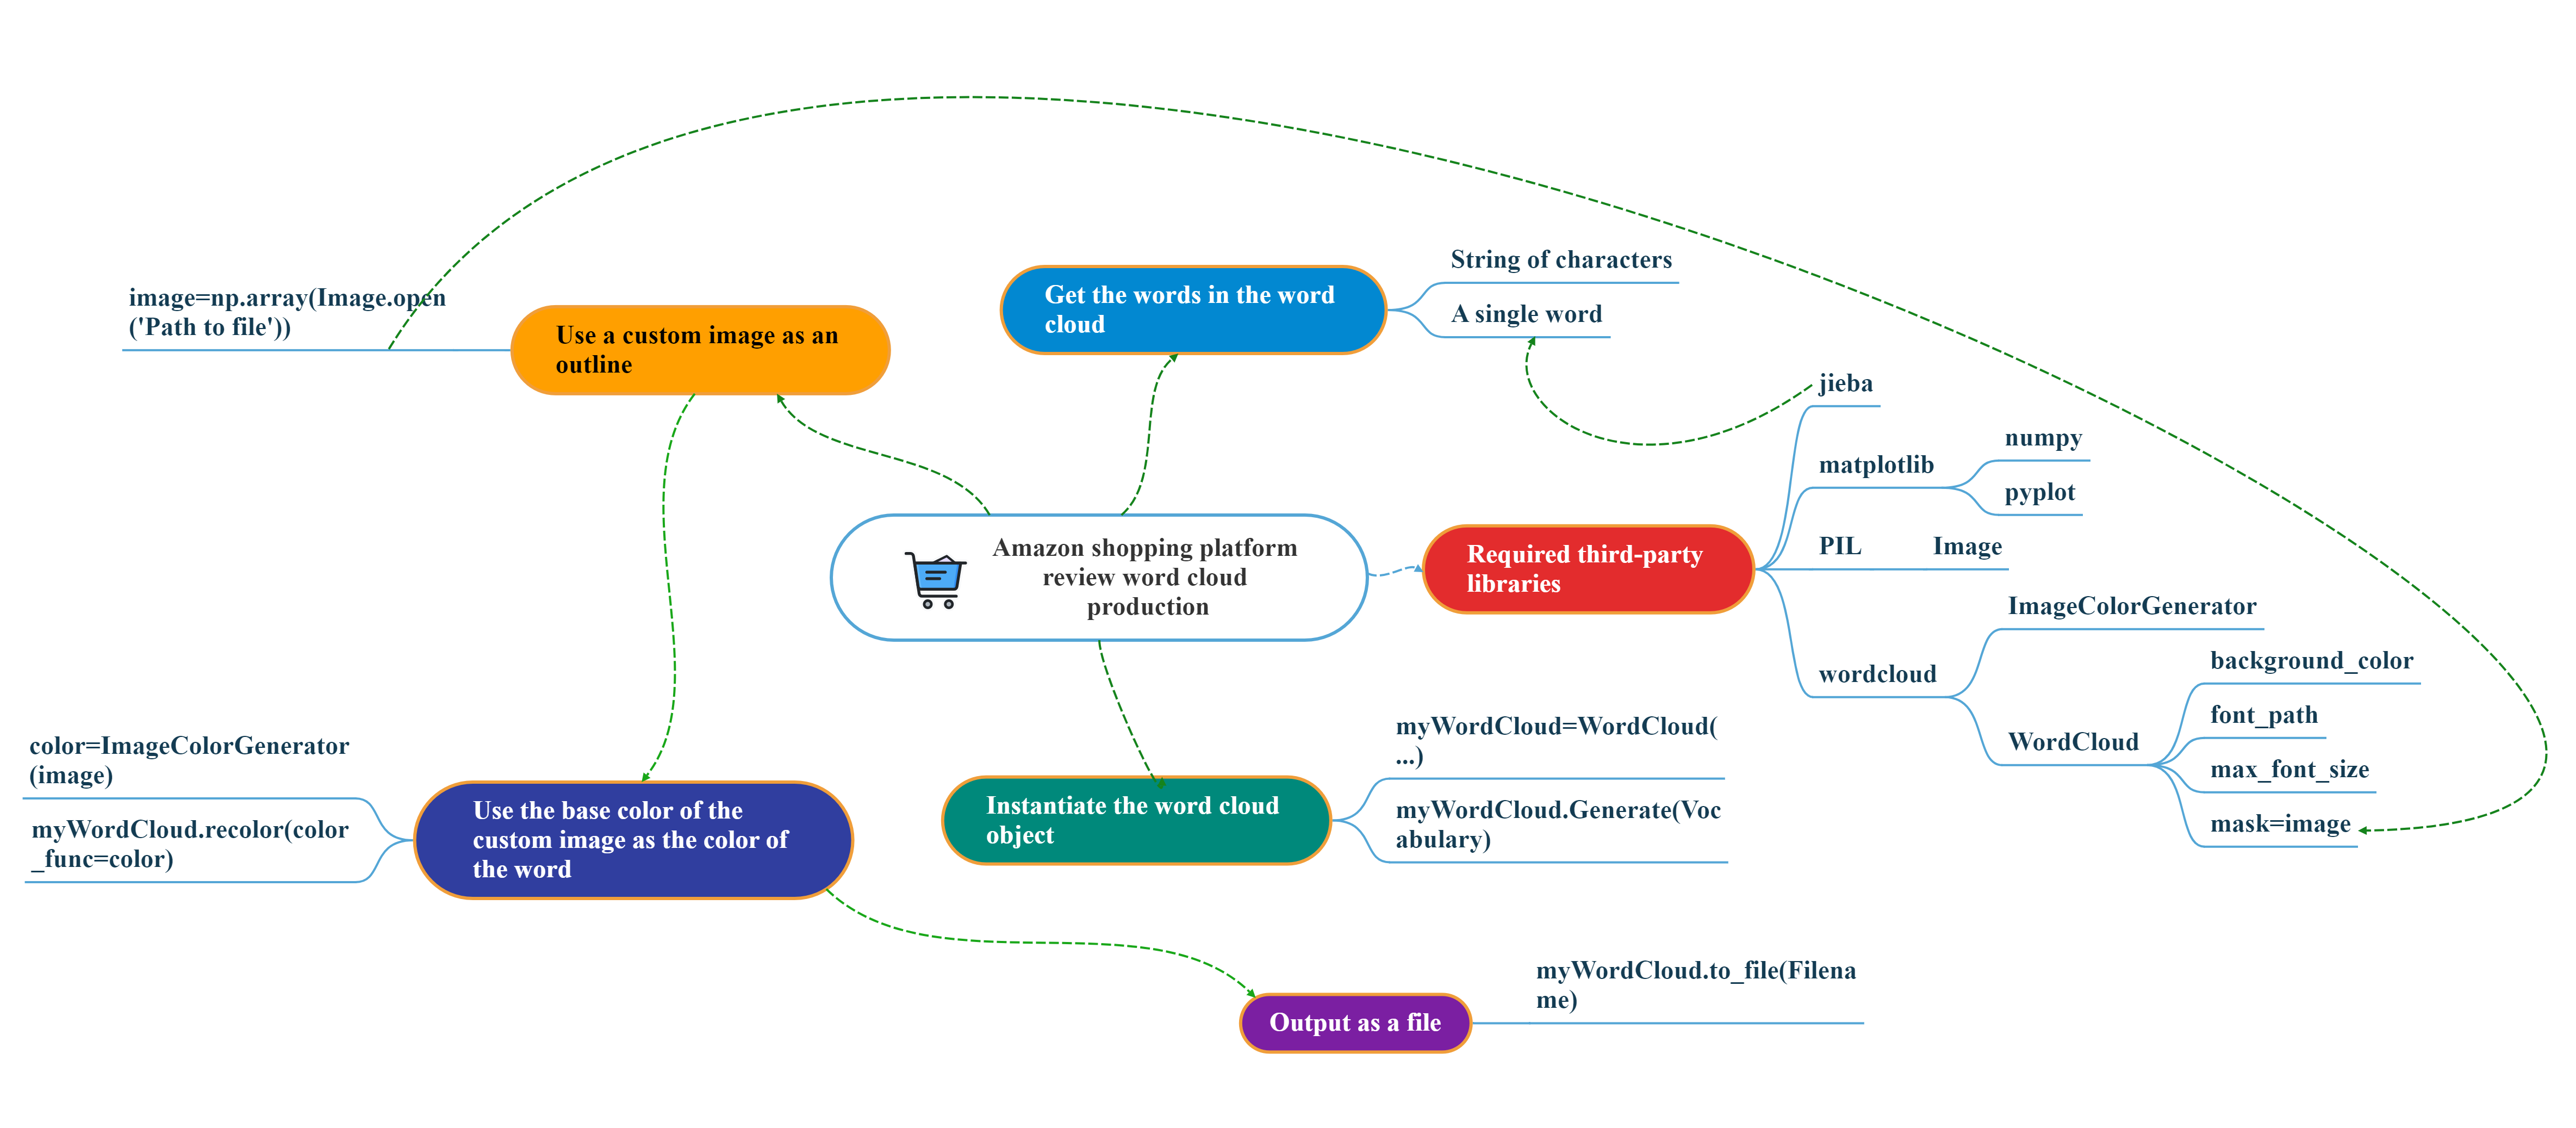
\includegraphics[width=16cm]{nlp1}
	\caption{Mind map of word cloud map generation algorithm}
	\label{nlp1}
\end{figure}
\subsection{Data Visualization and Analysis(Before Correction)}
In order to show the overall situation of the data as comprehensively as possible,we did not initially remove some pronouns, articles, and prepositions, after calculating the frequency of each word in Appendix I and Appendix II, we first analyzed the data in each annex separately, and took the top 30 frequency words to draw a pie chart. The overall situation is presented in the form of word composition and percentage respectively, as shown in Figure~\ref{nlp2} and Figure~\ref{nlp3}.Subsequently, the data in Appendix I and Appendix II are combined to draw the composite pie chart of the top 30 combined frequencies, and the top 10 words are listed separately, which reflects the objective situation of word frequency in the comments on the platform in a more macro way, as shown in Figure~\ref{nlp4}. At the same time, we take the top 100 words of Appendix I and II frequency and draw them in the form of weight heat map, and form an obvious correspondence, as shown in Figure~\ref{nlp5}, Figure~\ref{nlp6} and Figure~\ref{nlp7}.
\begin{figure}[H]
	\centering
	\begin{minipage}[t]{0.45\linewidth}
		\centering
		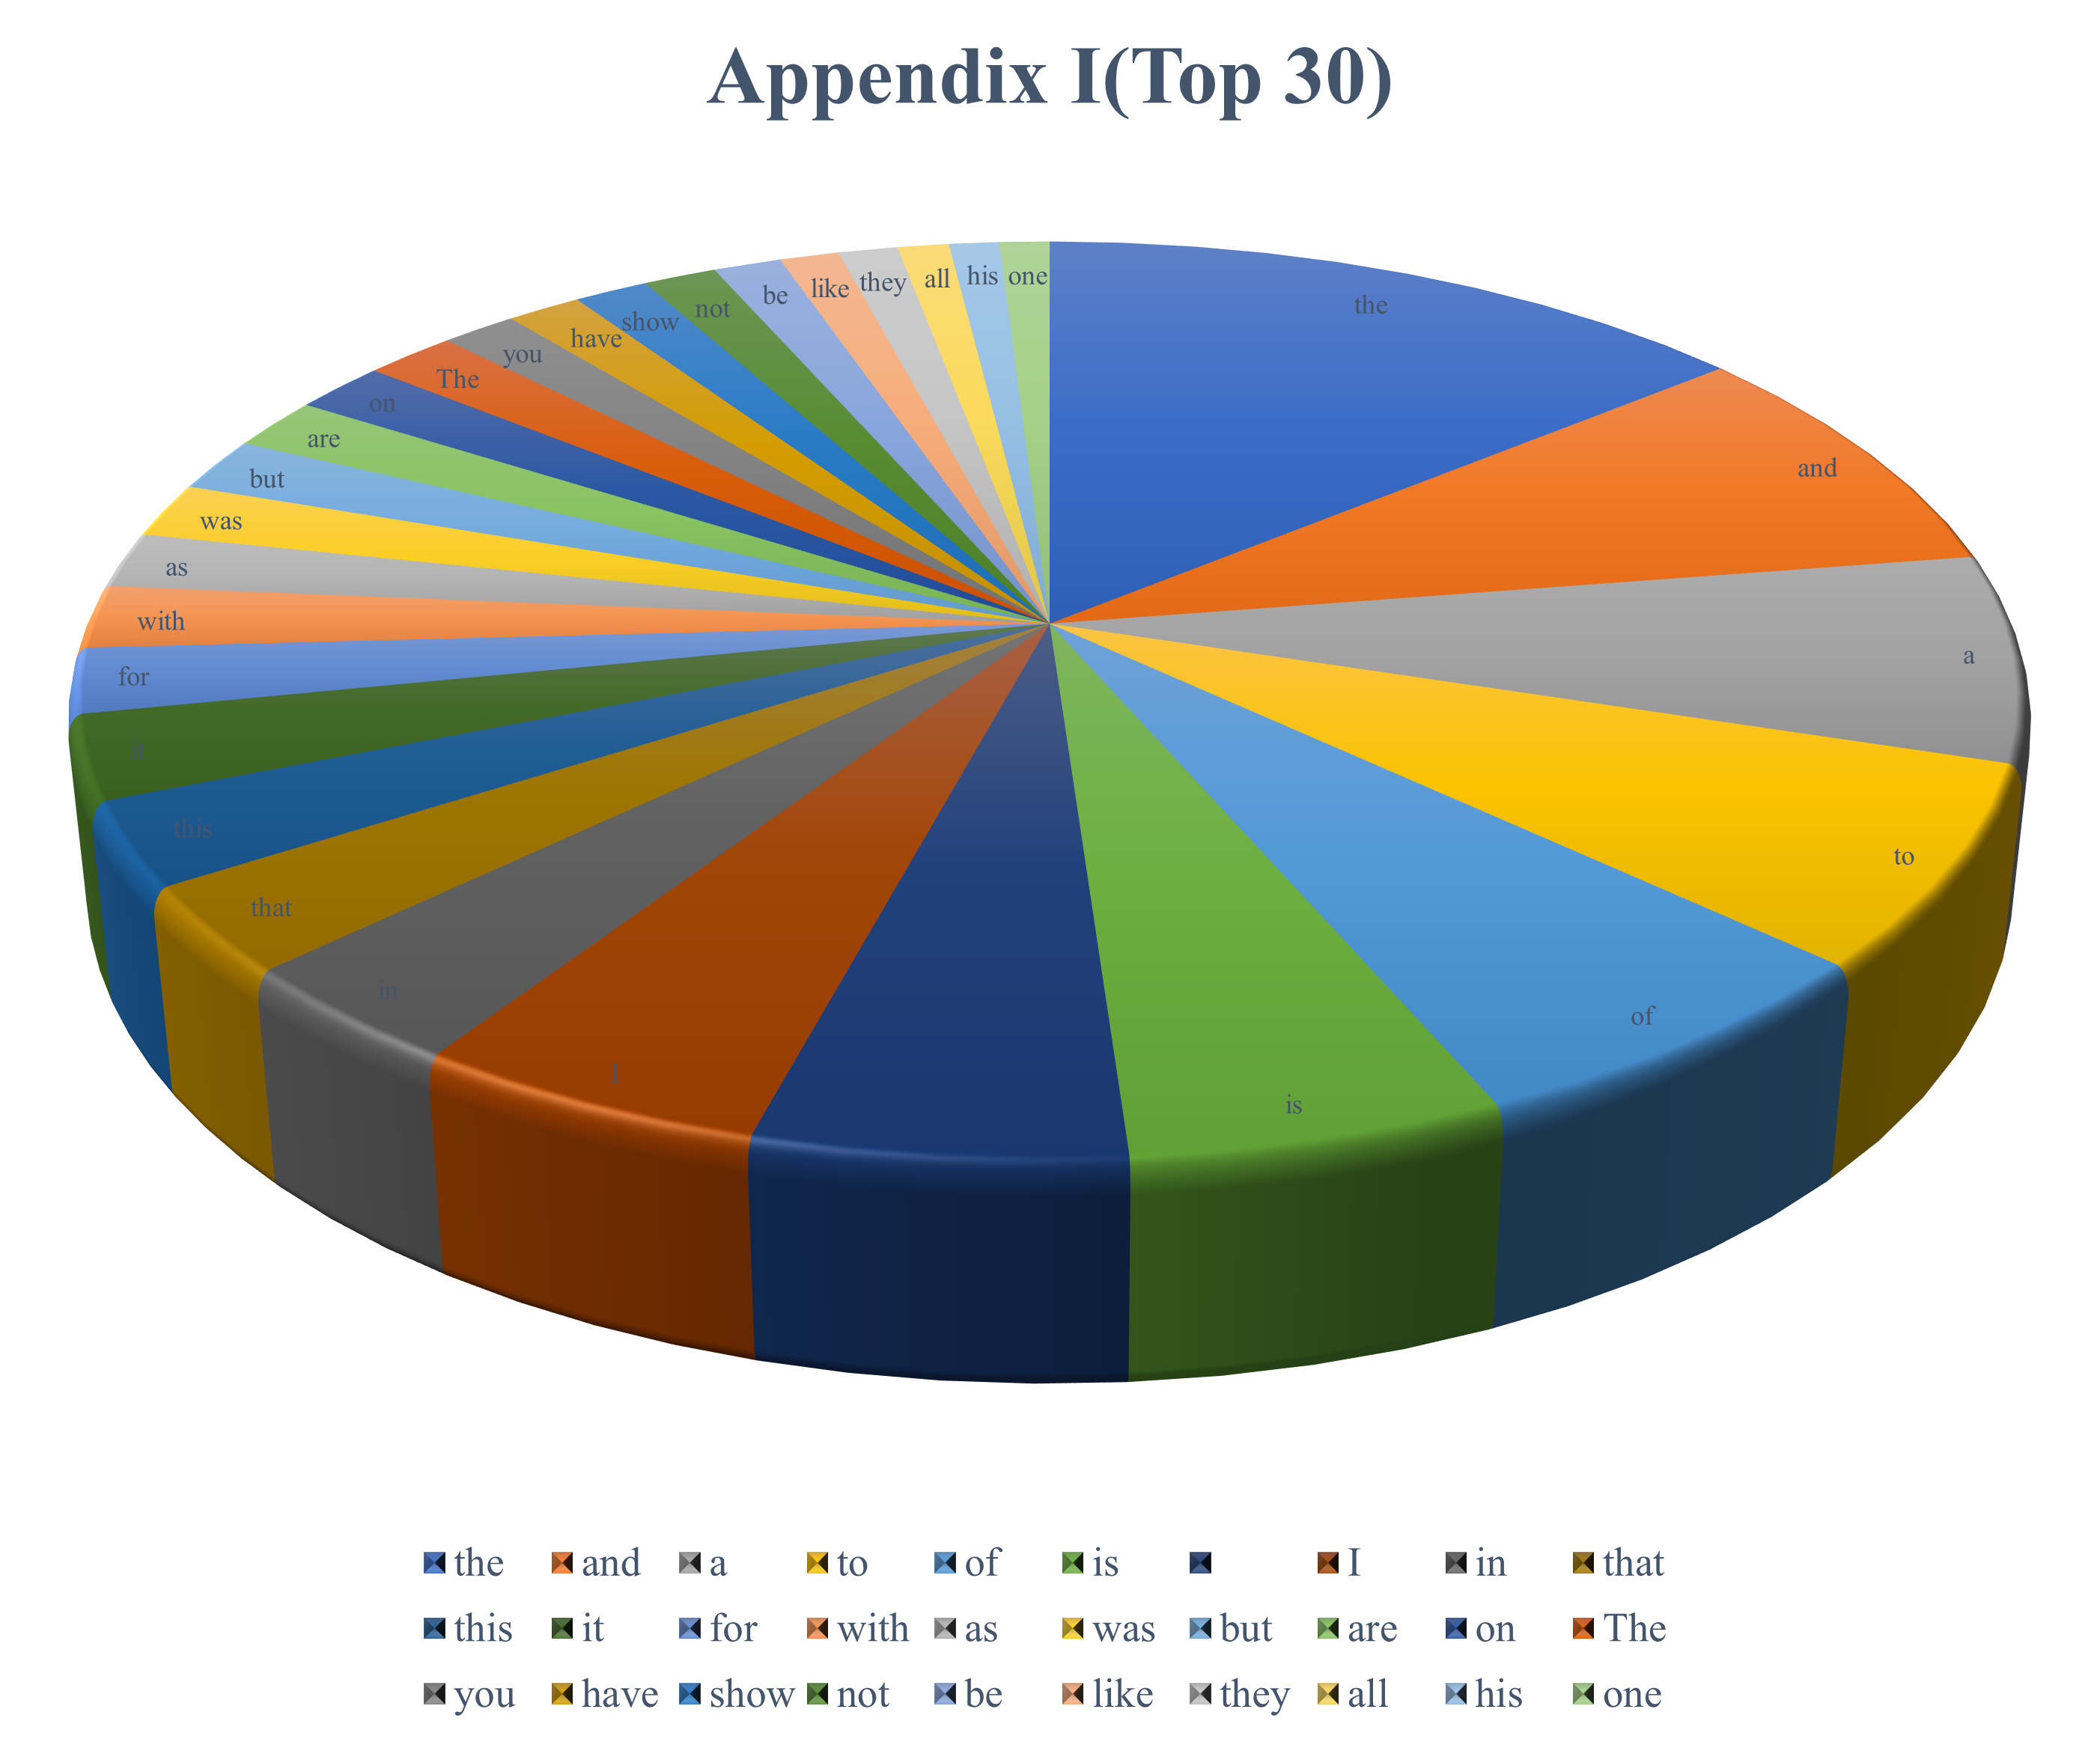
\includegraphics[width=7cm]{nlp2}
		\caption{Appendix 1 (Top30)}
		\label{nlp2}
	\end{minipage}
	\qquad
	\begin{minipage}[t]{0.45\linewidth}
		\centering
		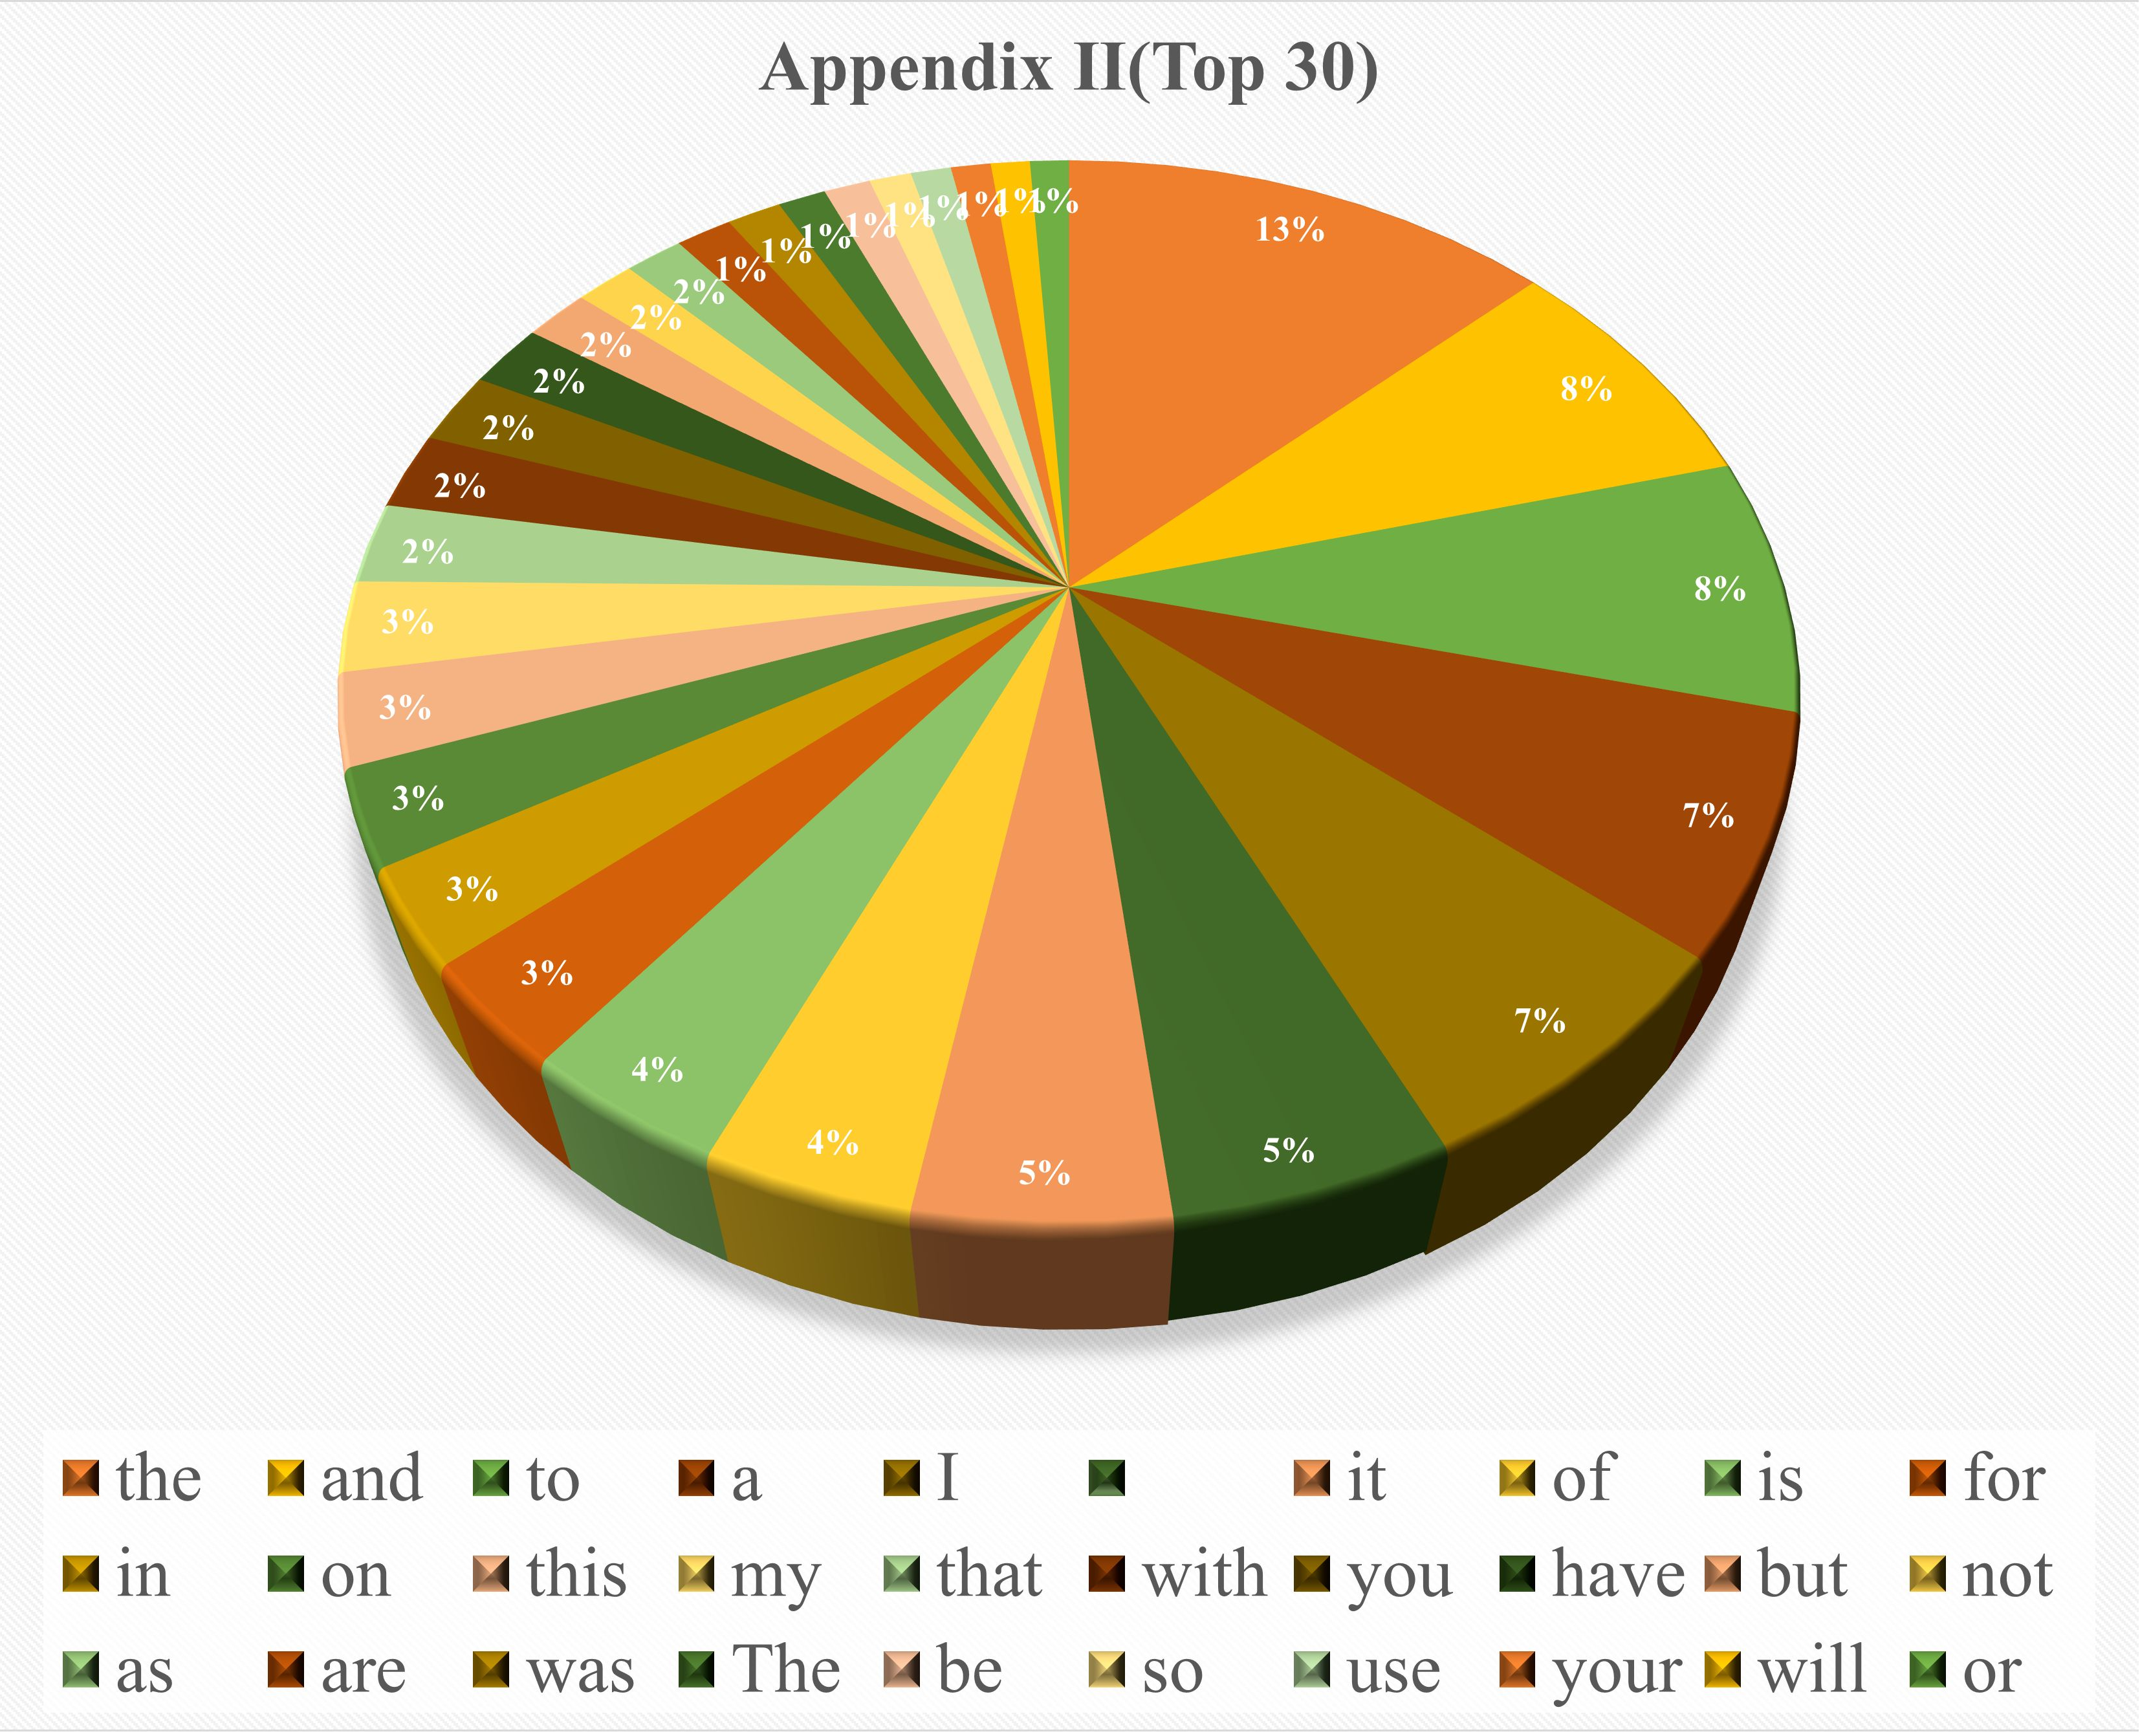
\includegraphics[width=7cm]{nlp3}
		\caption{Appendix 2 (Top30)}
		\label{nlp3}
	\end{minipage}
\end{figure}
\begin{figure}[H]
	\centering
	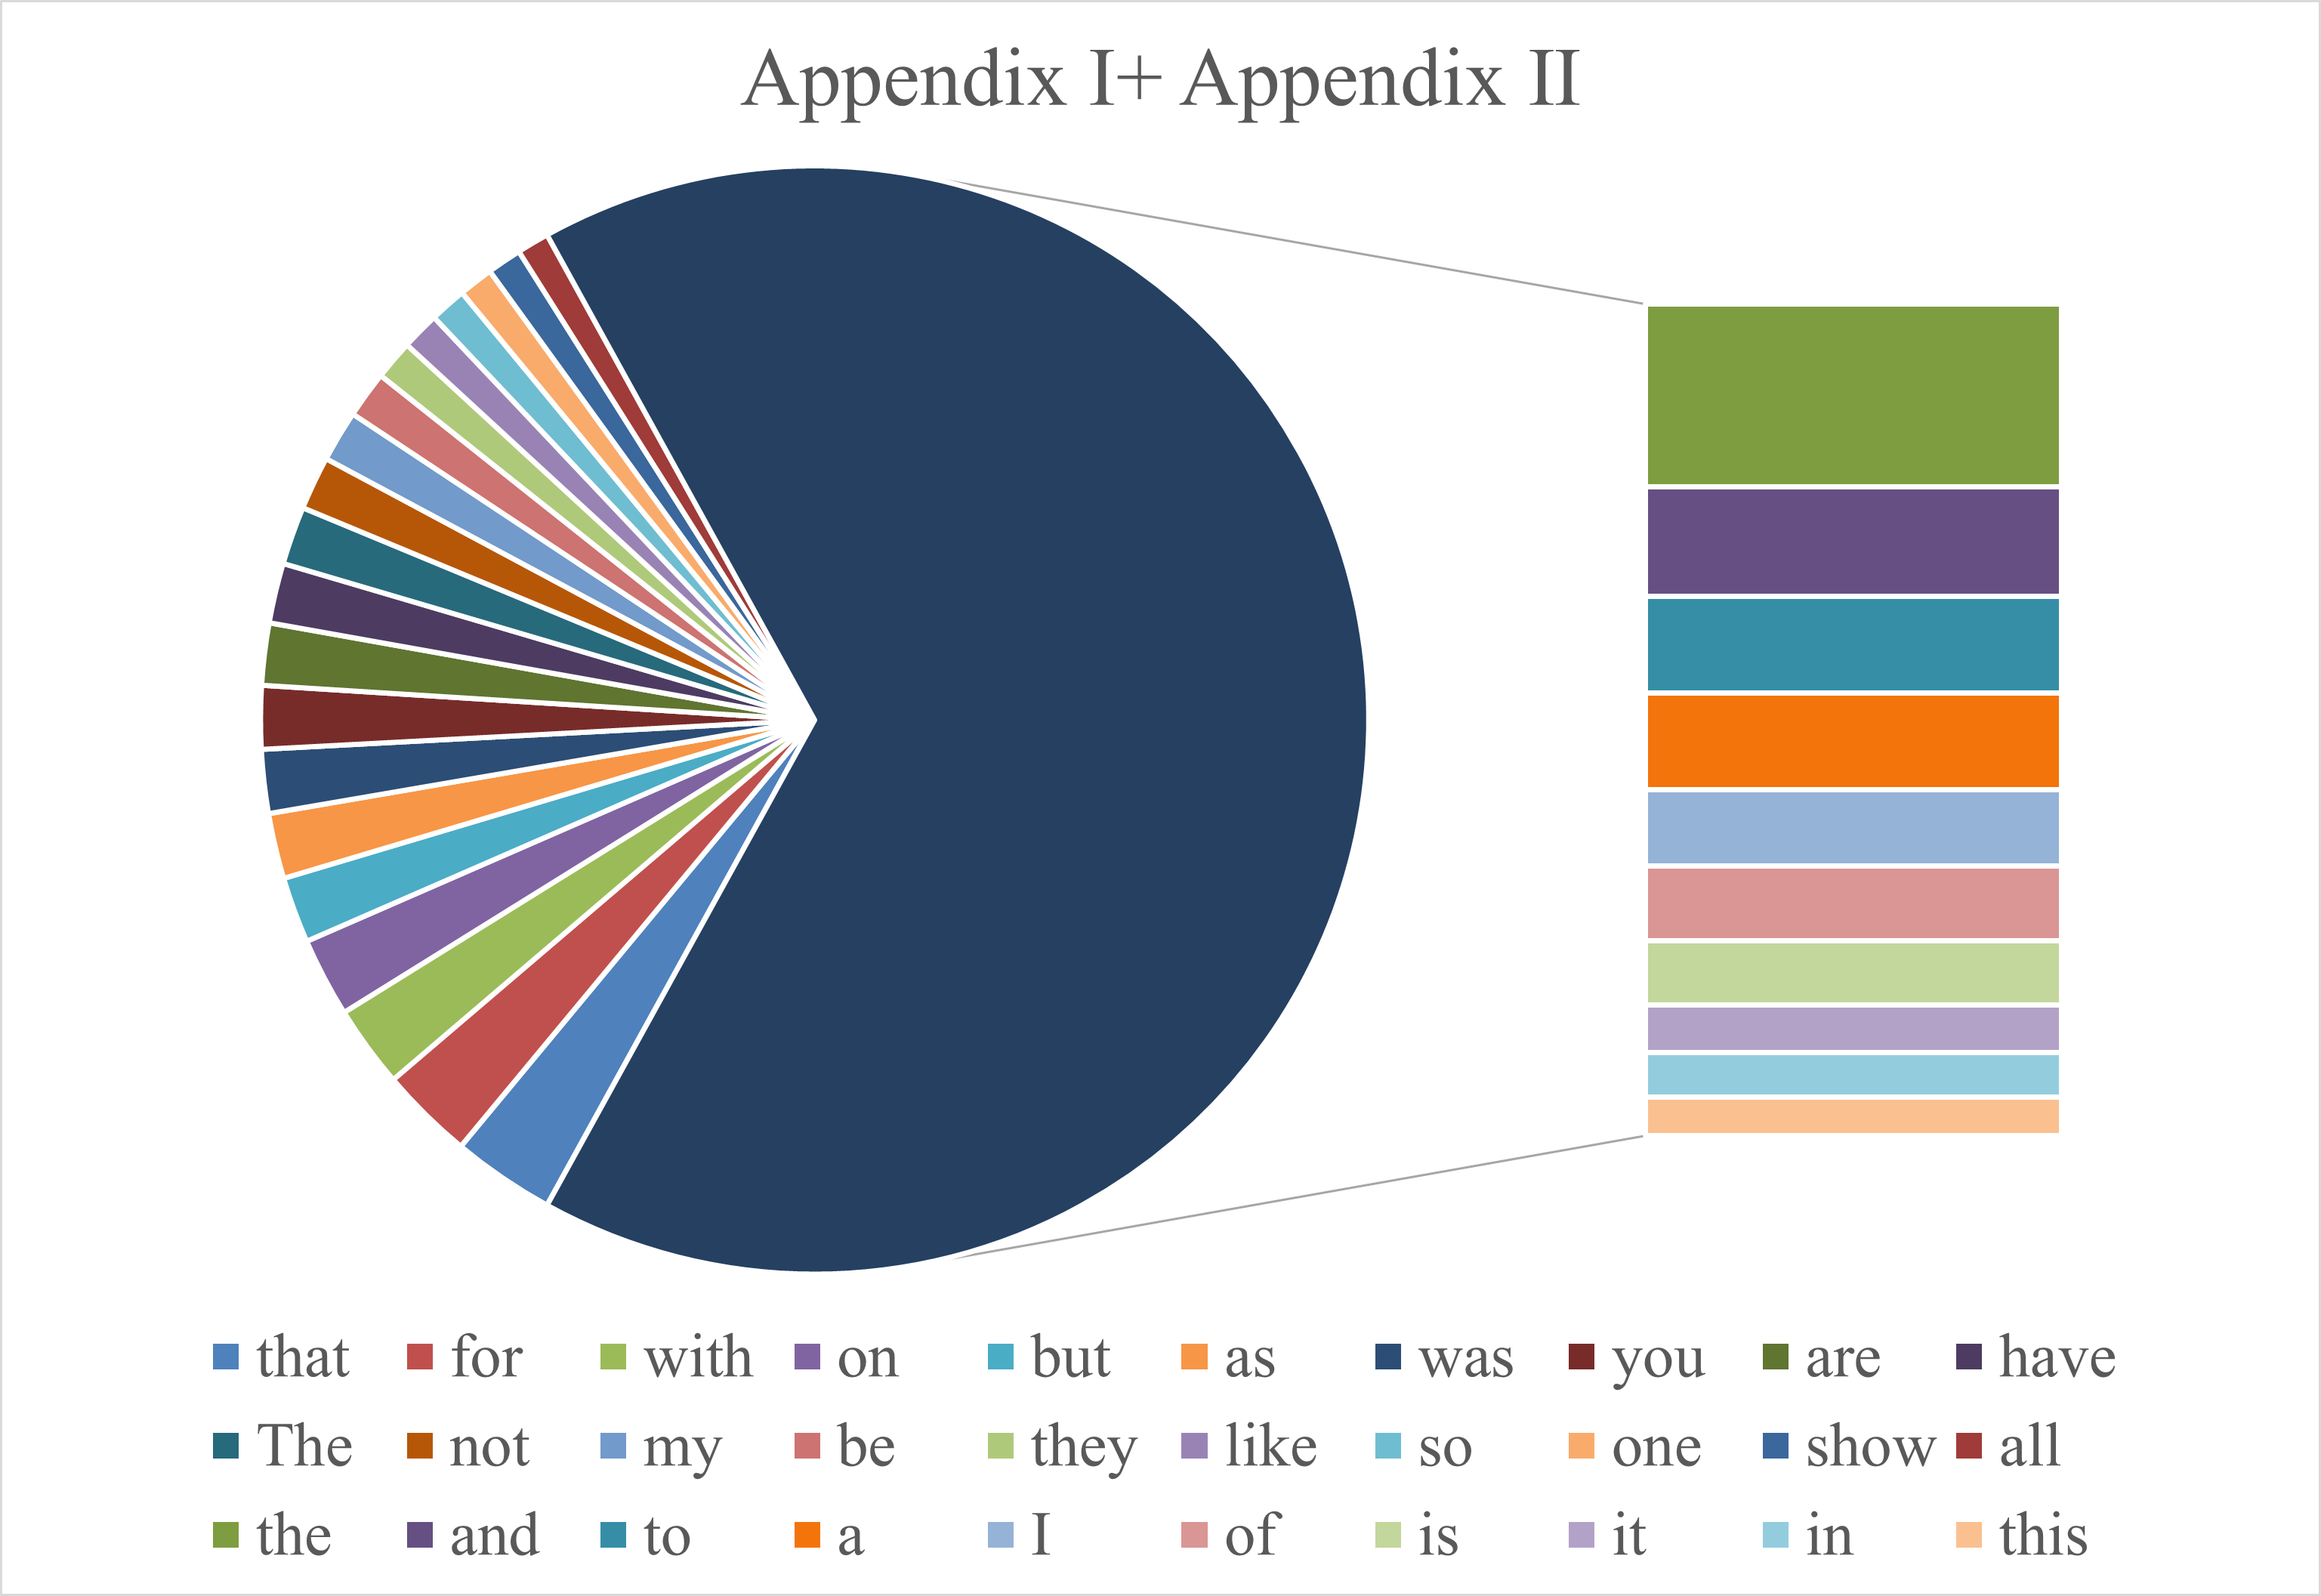
\includegraphics[width=14cm,height=9cm]{nlp4}
	\caption{Appendix 1+Appendix 2 (Top30)}
	\label{nlp4}
\end{figure}
As shown in Figure~\ref{nlp2},~\ref{nlp3} and~\ref{nlp4}, when we do not deal with stop words such as prepositions, pronouns and articles, the words with the highest frequency in user comments are basically ‘the,and,to,a,I,of ‘and other words that are inevitable in our daily life context, which is consistent with our life experience and vocabulary language characteristics.Therefore, we believe that our word frequency statistical model is reasonable and can be further used to count and rank informative and valuable words such as nouns and adjectives excluding stop words, so as to calculate the frequency of valuable words and draw a real word cloud map highlighting consumption views and emotional tendencies.
\begin{figure}[H]
	\centering
	\begin{minipage}[t]{0.45\linewidth}
		\centering
		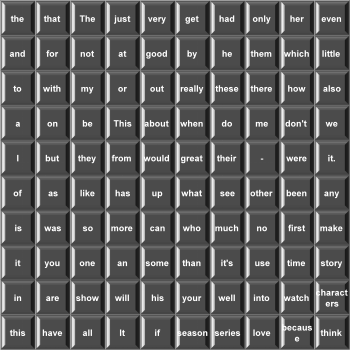
\includegraphics[width=7cm]{nlp5}
		\caption{Word Top 100}
		\label{nlp5}
	\end{minipage}
	\qquad
	\begin{minipage}[t]{0.45\linewidth}
		\centering
		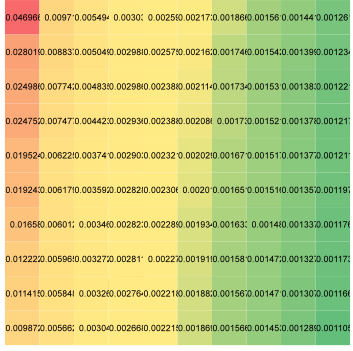
\includegraphics[width=7cm]{nlp6}
		\caption{The Frequency of Top 100}
		\label{nlp6}
	\end{minipage}
\end{figure}
\begin{figure}[H]
	\centering
	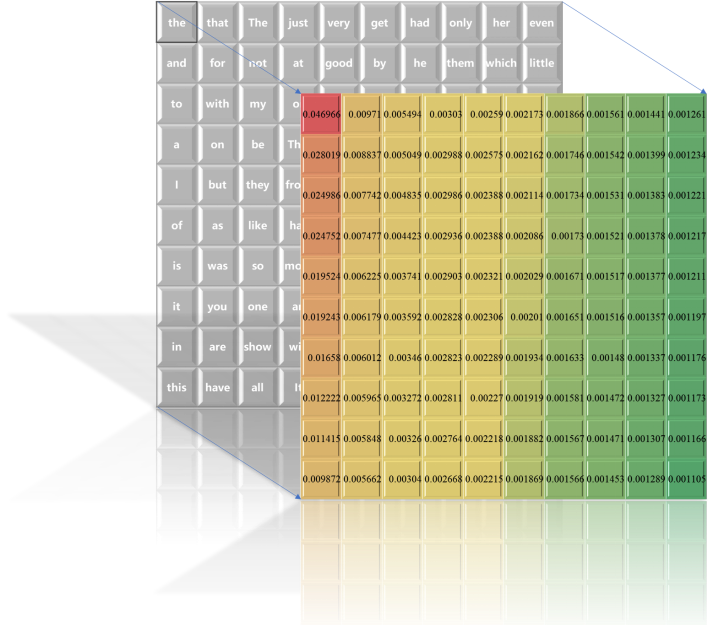
\includegraphics[width=14cm]{nlp7}
	\caption{One-to-One Correspondence between Words and Frequencies}
	\label{nlp7}
\end{figure}
\subsection{Data Visualization and Analysis(After Correction)}
On the previous page, we showed the frequency analysis of Appendix I and Appendix II without removing stop words, as shown in Figures~\ref{nlp5},~\ref{nlp6} and~\ref{nlp7}. The results show that the frequency is particularly small in the intuitive case, which leads to a large error. So in the case of removing stop words and missing values as well as numbers and punctuation marks (since question 1 focuses on text analysis and question 2 focuses on semantic analysis, here we present the details of the data processing in question 2), we use the number of frequencies instead of the proportion of frequencies, which greatly reduces the complexity. In this case we derive the frequency ranking as shown in Figures~\ref{nlp8} and~\ref{nlp9}.The word cloud plots is shown in Figures~\ref{nlp10} ,~\ref{nlp11},~\ref{nlp12}and~\ref{nlp13}.
\begin{figure}[H]
	\centering
	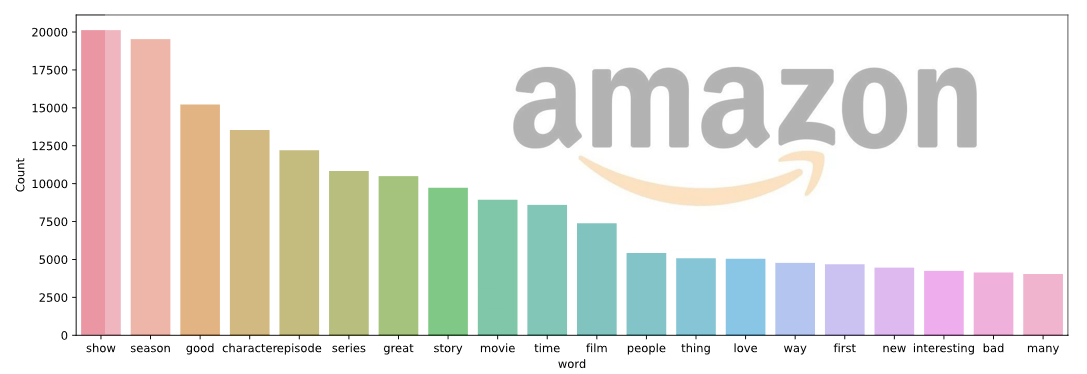
\includegraphics[height=4.8cm]{nlp8}
	\caption{Appendix 1(The Corrected Top 20)}
	\label{nlp8}
\end{figure}
\begin{figure}[H]
	\centering
	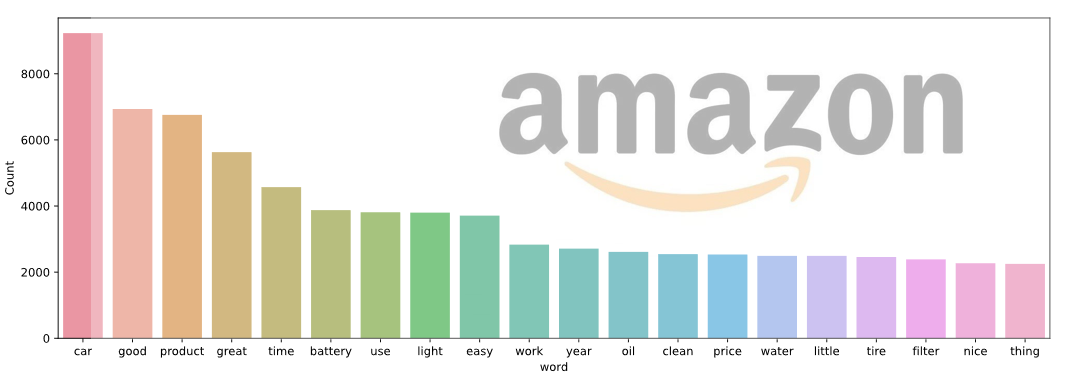
\includegraphics[height=4.8cm]{nlp9}
	\caption{Appendix 2(The Corrected Top 20)}
	\label{nlp9}
\end{figure}
According to Figure~\ref{nlp8}, from these high-frequency words, we can see that reviewers generally pay attention to TV series, movies and other forms of entertainment content (such as show, season, episode, series, movie, film, etc.). In addition, reviewers focus on the quality of the content (e.g., good, great, interesting, bad, etc.), as well as the storyline and characters (e.g., character, story, people, etc.).According to Figure~\ref{nlp9}, from these high-frequency words, we can see that reviewers generally pay attention to car-related products and services (such as car, battery, oil, tire, filter, etc.). In addition, reviewers also focus on the quality of the product (e.g., good, great, nice, etc.), the experience of using the product (e.g., easy, work, etc.), and the price (e.g., price). Reviewers also mentioned words related to car maintenance (clean, water, etc.).
\begin{figure}[H]
	\centering
	\begin{minipage}[t]{0.45\linewidth}
		\centering
		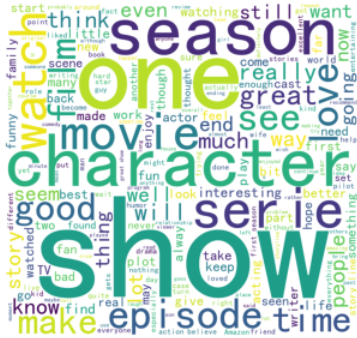
\includegraphics[height=5.2cm]{nlp10}
		\caption{Word Cloud Map 1(n.,adj.,v.)}
		\label{nlp10}
	\end{minipage}
	\begin{minipage}[t]{0.45\linewidth}
		\centering
		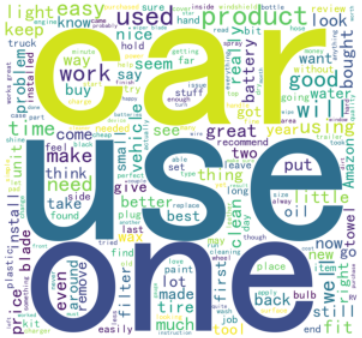
\includegraphics[height=5.2cm]{nlp11}
		\caption{Word Cloud Map 2(n.,adj.,v.)}
		\label{nlp11}
	\end{minipage}
\end{figure}
\begin{figure}[H]
	\centering
	\begin{minipage}[t]{0.45\linewidth}
		\centering
		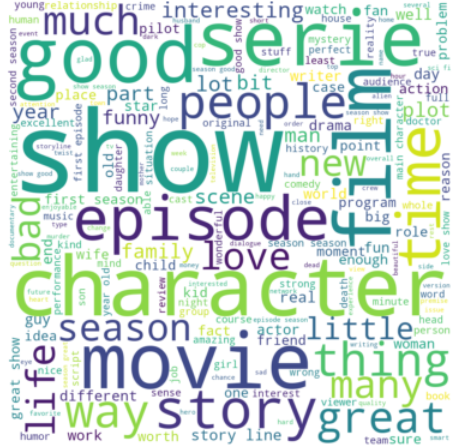
\includegraphics[height=5.2cm]{nlp12}
		\caption{Word Cloud Map 1(n.,adj.)}
		\label{nlp12}
	\end{minipage}
	\begin{minipage}[t]{0.45\linewidth}
		\centering
		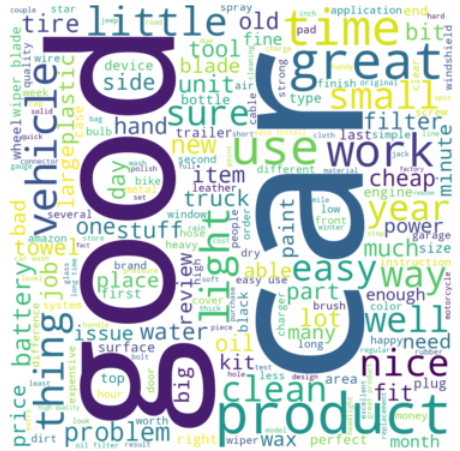
\includegraphics[height=5.2cm]{nlp13}
		\caption{Word Cloud Map 2(n.,adj.)}
		\label{nlp13}
	\end{minipage}
\end{figure}
\section{Task 2: Semantic Analysis of Commodity Reviews}
\subsection{General Idea Analysis}
\label{sec5.1}
In order to perform semantic analysis and infer product names, we first preprocess the data and observe that a large part of the data in Appendix III and Appendix IV are invalid information. The only useful information for us is reviewtext and summary. This is because each asin corresponds to an item on the Amazon platform, but products with different asin codes may also belong to the same class. Only nouns and adjectives remain after data processing, which is convenient for our further analysis.

In order to perform semantic analysis and infer product names, we first preprocess the data and observe that a large part of the data in Appendix III and Appendix IV are invalid information. The only useful information for us is reviewtext and summary. This is because each asin corresponds to an item on the Amazon platform, but products with different asin codes may also belong to the same class. Only nouns and adjectives remain after data processing, which is convenient for our further analysis.

The LDA-K-TF-IDF model first uses the text mining ability of LDA to model the vocabulary in the document, and divides the vocabulary into multiple topics. Then, K-means clustering is used to cluster the words into multiple clusters, and TF-IDF is used to extract the n most frequent words in each topic and cluster them. Then, by adjusting the number of topics and clusters, the overlap degree of n words in the two models is the highest (the proportion of common words in n words). By keeping each parameter unchanged and taking the intersection, we can obtain the product name of each asin.
\subsection{Review Data Preprocessing}
Before the semantic analysis of the product review text, we first need to preprocess the data, because we want to establish a mathematical model of semantic analysis, in order to extract the keywords in the review, so as to carry out the theme analysis, to achieve the purpose of infering the product name according to the content of the product review.

As we know from our daily life experience, the ID and name of each person and the number of the product have no correlation with the content of the product, and the time of each person's comment on the product is not helpful for us to reason about the product name. The content and summary of each person's comment are based on the cognition and feeling of using the product, which makes us make the highest priority indicator. So we first need to remove the content such as reviewerID, asin, helpful, overall, unixReviewTime, reviewTime, etc. and only use the content of reviewText and summary for modeling and text mining.

According to the analysis results of question 1, the most common words in the comment text are ‘the,and,to,I,a,’ such as articles, prepositions, pronouns, punctuation marks and numbers, etc. These words are not helpful for our modeling, so we should also remove them, so as to further remove the noise in the text after processing. We use lemmatization from spacy to return the word to its original form, reduce the repetition of the word tokenize the comment, then lemmatize it, not only restoring the word form, but also leaving only nouns and adjectives. After that, we transform the word into its normal form. In this way, we have completed the preprocessing of the data and can conduct topic modeling.
\begin{figure}[H]
	\centering
	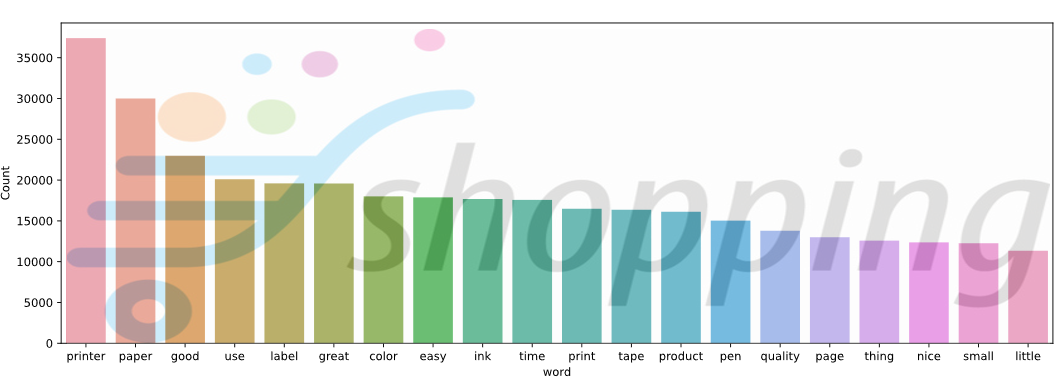
\includegraphics[width=15cm]{nlp14}
	\caption{Data Processing Results (Take Appendix 3 as an Example)}
	\label{nlp14}
\end{figure}
\subsection{LDA (Latent Dirichlet Allocation)}
\label{sec5.3}
\subsubsection{Analysis of Model Principle}
LDA (Latent Dirichlet Distribution) is a generative topic model, and we assume Appendix III is a mixture of multiple topics, each of which in turn consists of multiple words. The goal of the LDA model is to infer the distribution of topics in that file and the distribution of words in each topic based on the Appendix III collection.

Choose parameter $\theta\sim p(\theta)$ ;

For each  $N$ of the  words $w_n$ :
\begin{itemize}
\item Choose a topic $z_n\sim p(z|\theta)$ ;
\item Choose a word $w_n\sim p(w|z)$ ;
\end{itemize}

Where $\theta$ is a topic vector, and each column of the vector represents the probability of each topic appearing in Appendix III. The vector is a nonnegative normalized vector. $p(\theta)$ is the distribution of $\theta$, specifically Dirichlet distribution, that is, the distribution of distributions;  $z_n$represents the selected topic,  $p(z|\theta)$represents the probability distribution of topic  $z$ given $\theta$ , specifically the value of $\theta$, which is $p(z=i|\theta)=\theta_{i}$ .

This method first selects a topic vector $\theta$ and determines the probability of each topic being selected. Then, when generating the inner word, a topic $z$ is selected from the topic distribution vector $\theta$ , and a word is generated according to the word probability distribution of topic $z$.\cite{2}\cite{3}The graph model is shown as follows:
\begin{figure}[H]
	\centering
	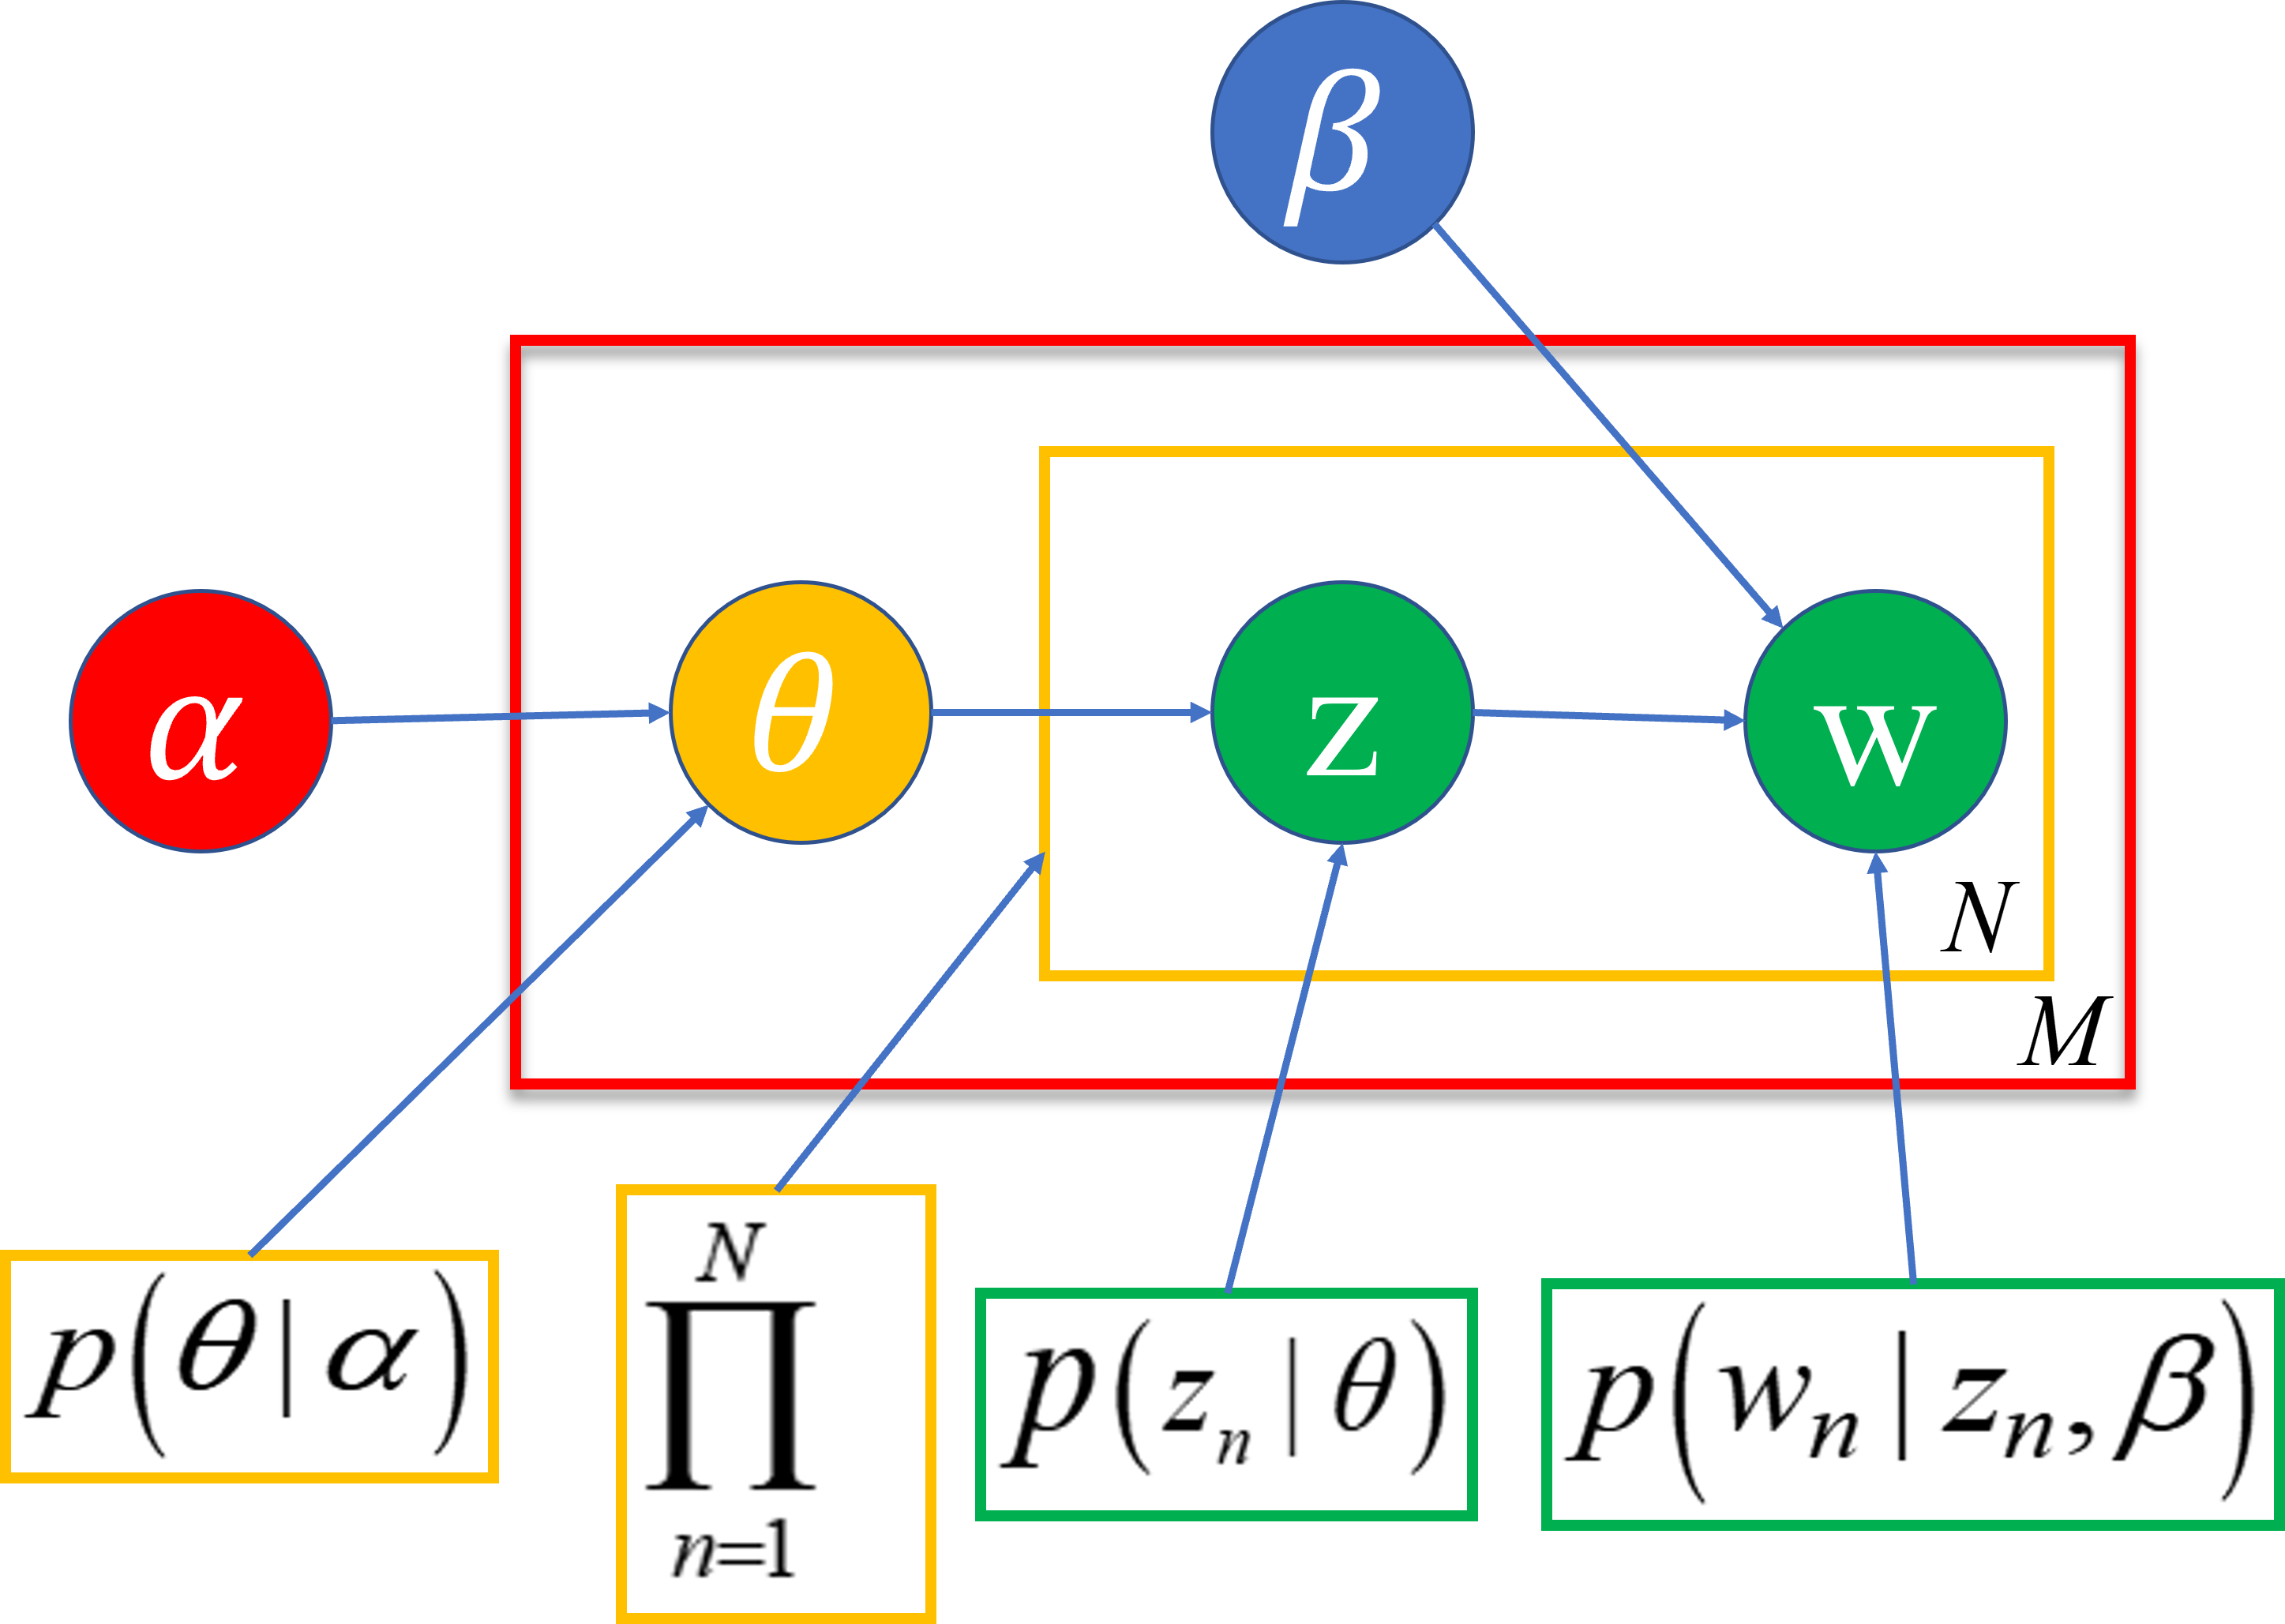
\includegraphics[width=10cm,height=6cm]{nlp15}
	\caption{A Graph Model of LDA}
	\label{nlp15}
\end{figure}
From the figure above, we can see the joint probability of LDA:
\begin{equation}
	p(\theta,z,w | \alpha,\beta)=p(\theta|\alpha)\prod_{n=1}^{N}p=(z_n|\theta)p(w_n | z_n,\beta)
\end{equation}
For ease of understanding, the three presentation layers of LDA are shown in three colors:
\begin{itemize}
\item Corpus-level (red) : $\alpha$ and $\beta$ indicate the corpus-level parameters, i.e. each document is the same, so the generation process will only sample once.
\item Document-level (orange) : $\theta$ is a variable at the document level, with an $\theta$ for each document, which means that each document has a different probability of producing each topic $z$ , so generate a $\theta$ for each document.
\item Word-level (green) :  $z$ and $w$ are both word-level variables, $z$ is generated from $\theta$, $w$ is generated from $z$ and $\beta$ together, and a word $w$ corresponds to a topic $z$.
\end{itemize}
From the above discussion on the LDA generation model, it can be known that the LDA model mainly learns and trains two control parameters  $\alpha$ and $\beta$  from the given input corpus. After learning these two control parameters, the model is determined and can be used to generate documents. Where $\alpha$ and  $\beta$ correspond to each of the following information:
\begin{itemize}
	\item $\alpha$ The distribution $p(\theta)$ requires a vector parameter, the parameter of the Dirichlet distribution, for generating a topic $\theta$ vector;
	\item $\beta$ Probability distribution matrix of words for each topic $p(w|z)$.
\end{itemize}
Considering $w$ as the observed variable and $\theta$ and $z$ as the hidden variable, $\alpha$  and $\beta$ can be learned by EM algorithm. In the process of solving, the posterior probability $p(\theta,z|w)$ cannot be directly solved, so a lower bound of likelihood function is needed to approximate the solution. This can be computed using variational inference based on factorization assumptions, using the EM algorithm. Each time the E-step inputs $\alpha$ and $\beta$, compute the likelihood function, the M-step maximizes this likelihood function, compute $\alpha$ and $\beta$, and iterate until convergence.
\subsubsection{Programming Implementation and Visualization of Results}
\begin{figure}[H]
	\centering
	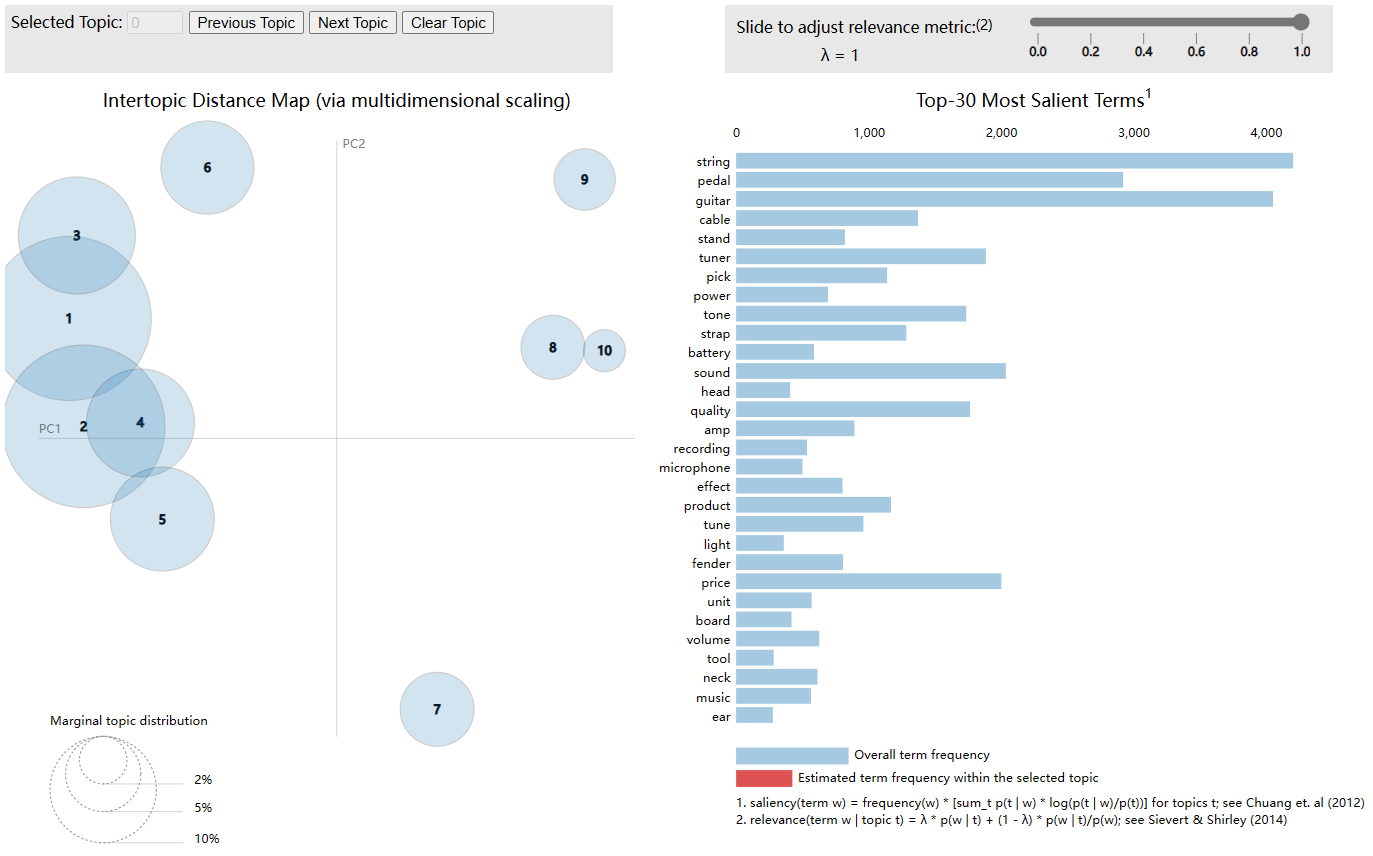
\includegraphics[width=14cm,height=7cm]{nlp16}
	\caption{ Interactive Visualization of Topic Modeling Data}
	\label{nlp16}
\end{figure}
Before visualizing the data, we ran the program and found that a thorough topic modeling of the data in the appendix would generate 2,420 topics. Due to the time complexity of the code and the space complexity of the vector plots, we found that the amount of data in Appendix III and Appendix IV would generate 900 topics. Because we need to specify the number of topics generated during the execution of the algorithm, that is, the $num\_topics$ parameter needs to be set manually, we first calculate the $asin$ code in Appendix IV. The same $asin$ code is the same product, but different $asin$ codes also have the possibility of the same product, too few topics will increase the error. However, too many topics can lead to overfitting, so we adjusted the parameter and got a good result with $num\_topics$=100 for visualization.The topic distribution is shown in Figure~\ref{nlp16}. The processing method is the same in Appendix III, and the final results will be shown in Section~\ref{sec5.5}.The data visualization on the previous page is interactive, but because it is an html file, it can only be opened and manipulated on a web page, so we only show the overall picture of the subject.
\subsection{K-means Clustering Algorithm}
\subsubsection{Analysis of Model Principle}
After the problem analysis in Part~\ref{sec5.1}, it can be known that the data in Appendix III and Appendix IV belong to the training set without labels, so the supervised learning method is not feasible to some extent. We intend to use K-means clustering in unsupervised learning to vectorize the text data and then reduce the dimension. In k-means clustering, without knowing any sample labels in advance, the samples are divided into several categories through the internal relationship between the data, so that the similarity between samples of the same class is high and the similarity between samples of different classes is low (that is, the class cohesion is increased and the distance between the classes is reduced). Its core idea is to iteratively find a partitioning scheme for the K clusters that minimizes the loss function corresponding to the clustering result\cite{4}. We first perform the convergence proof, where the loss function can be defined as follows:
\begin{equation}
	J=\sum_{i=1}^{C}\sum_{j=1}^{N}r_{ij}\cdot v(x_j,\mu_i)
\end{equation}
Where is:
\begin{equation}
	v(x_j,\mu_i)=\parallel x_j-\mu_i\parallel^2,r_{nk}=
	\begin{cases}
		1 & \text{if} x_n\in k,\\
		0 & \text{else.}
	\end{cases}
\end{equation}
To find the extremum, we set the partial derivative of the loss function equal to 0:
\begin{equation}
	\frac{\partial J}{\partial \mu_k}=2\sum_{i=1}^{N}r_{ik}(x_i-\mu_k)=0
\end{equation}
When k is the KTH center, we have:
\begin{equation}
	\mu_k=\frac{\sum_{i=1}^{N}r_{ik} x_i}{\sum_{i=1}^{N}r_{ik}}
\end{equation}
It can be seen that the new center point is the centroid of all the classes.

The core goal of k-means is to partition a given dataset into K clusters (where K is a hyperparameter) and give a center point corresponding to each sample. The steps can be divided into four steps:
\begin{enumerate}
	\item Data preprocessing. Here we vectorize the text data in Appendix IV numerically and then preprocess the data.
	\item Randomly select K centers, denoted as:$\mu_1^{(0)}$,$\mu_2^{(0)}$,$\cdots$,$\mu_k^{(0)}$
	\item Define the loss function:$J(c,\mu)=\min\sum_{i=1}^{M}\parallel x_i-\mu_{c_i}\parallel^2$
	\item Let $t=0,1,2,\dots $ Is the number of iteration steps, repeat the following process until $J$ converges:
	\begin{itemize}
	    \item  For each sample $x_i$ , assign it to the nearest center $c_{i}^{t}<-\arg\min{k}\parallel x_i-\mu_{k}^{t}\parallel^2$
	    \item  For each center $k$, recalculate the center of the class$\mu_{k}^{(t+1)}<-\arg\min{\mu}\sum_{i:c_{i}^{t}=k}^{b}\parallel x_i-\mu\parallel^2$
	\end{itemize}
\end{enumerate}
\subsubsection{Programming Implementation and Visualization of Results}
In the programming implementation of the model solution, we first use the TF-IDF method to numerically vectorize the data processed text, and then specify the number of clusters. In order to be consistent with the LDA model topic parameters in Section~\ref{sec5.3}, we also use the parameter setting of n\_clusters=100 here. In order to show the results visually, we use principal Component Analysis (PCA) to reduce the dimension of TF-IDF matrix to two-dimensional space, and then draw a scatter plot, which effectively avoids the problem of inconsistent array size and retains the actual results of K-means clustering. The final clustering situation is shown in Figure~\ref{nlp18}. Good results are obtained.
\begin{figure}[H]
	\centering
	\begin{minipage}[t]{0.36\linewidth}
		\centering
		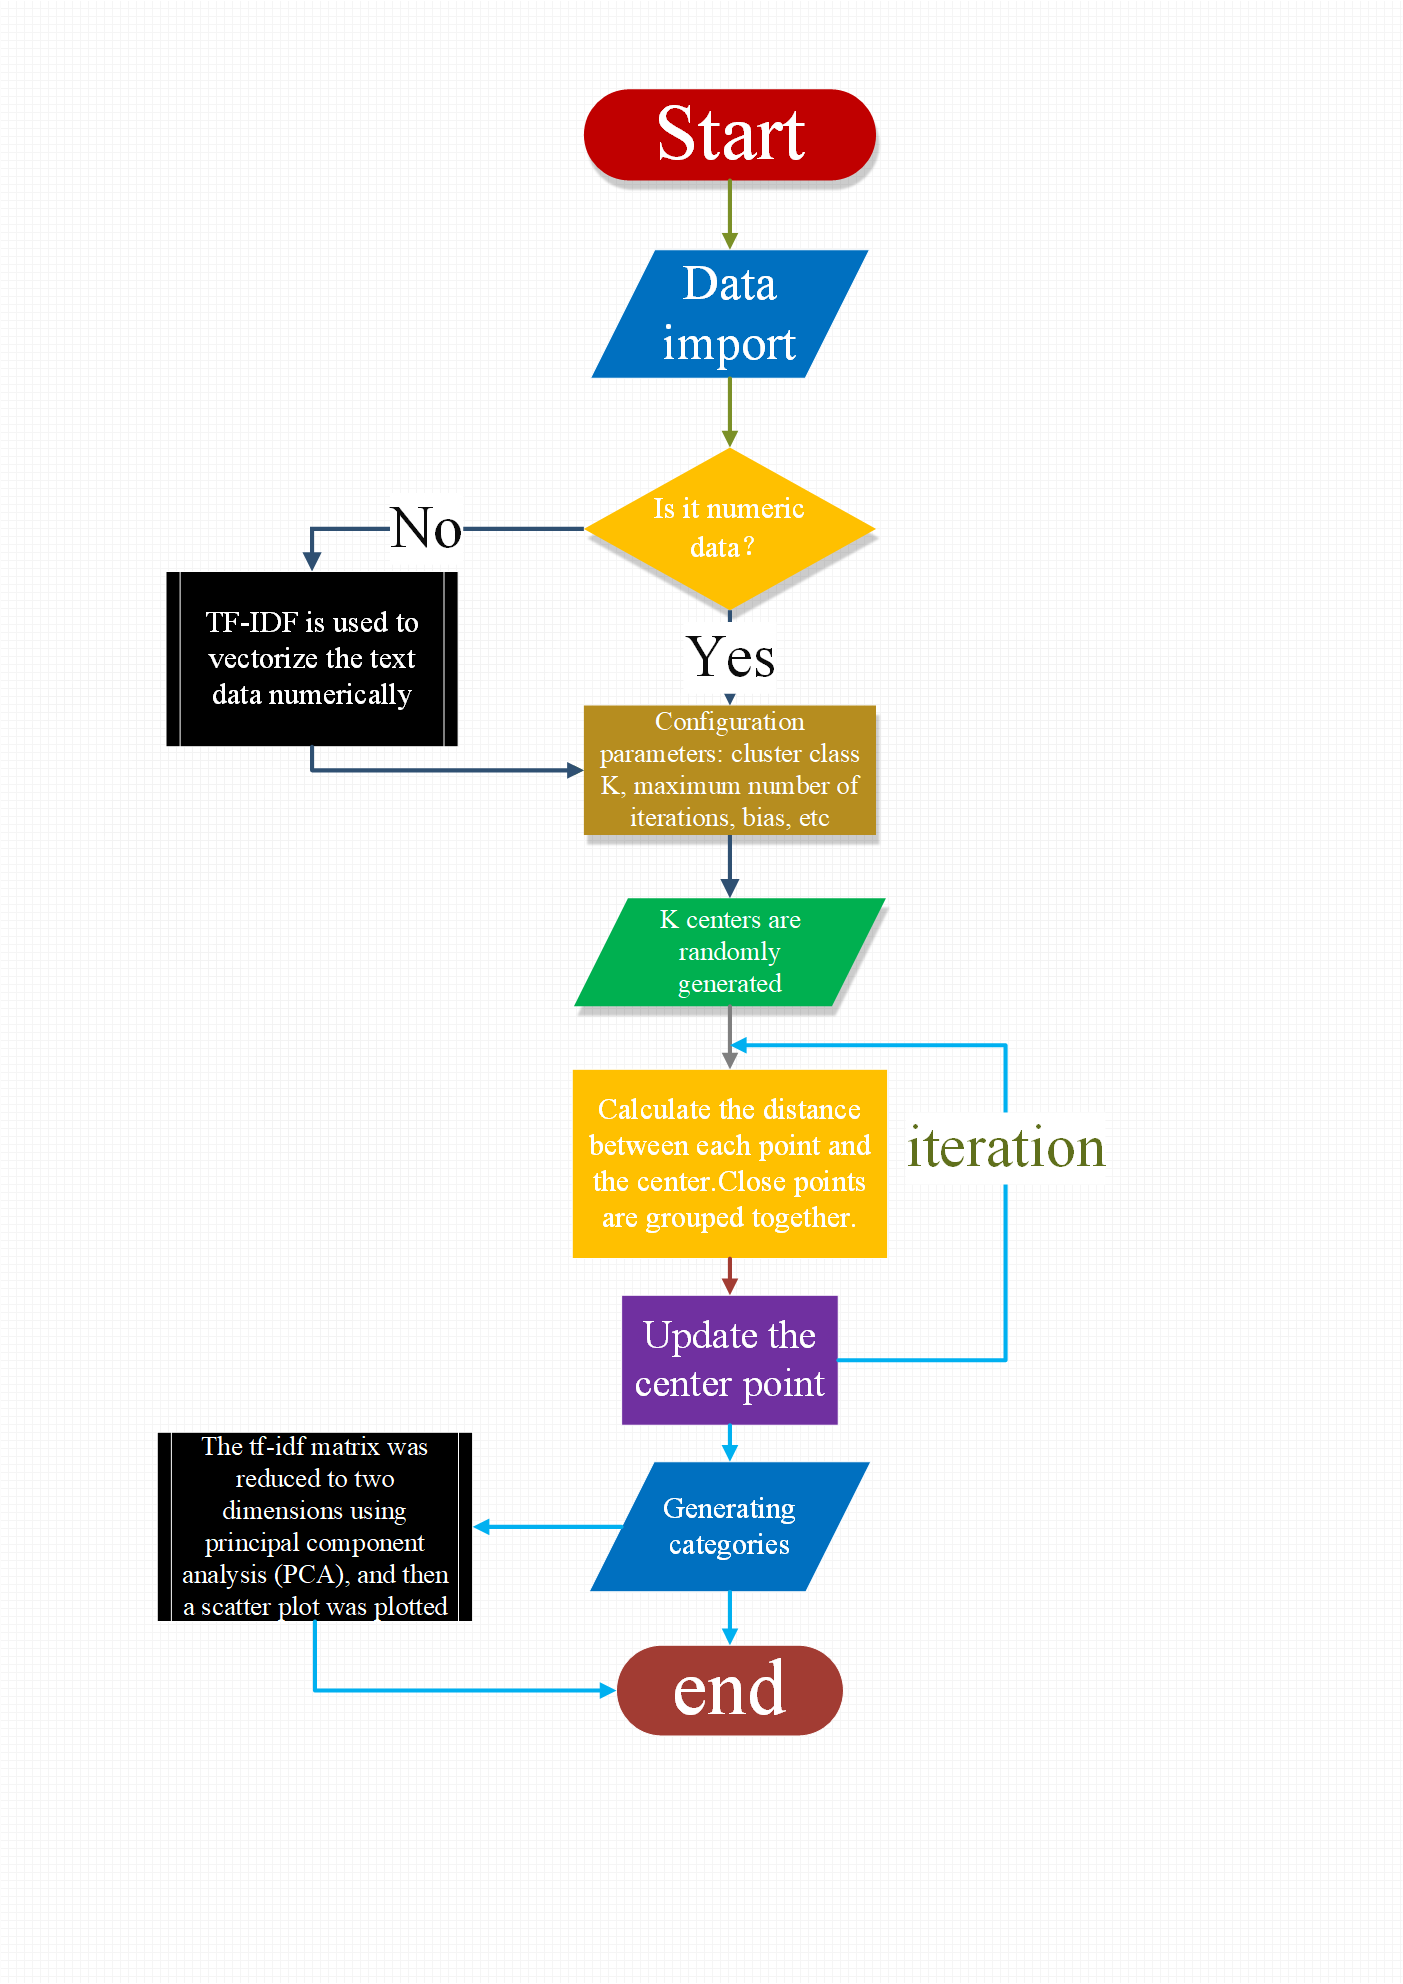
\includegraphics[width=5.5cm]{nlp17}
		\caption{K-Flow Chart}
		\label{nlp17}
	\end{minipage}
	\qquad
	\begin{minipage}[t]{0.54\linewidth}
		\centering
		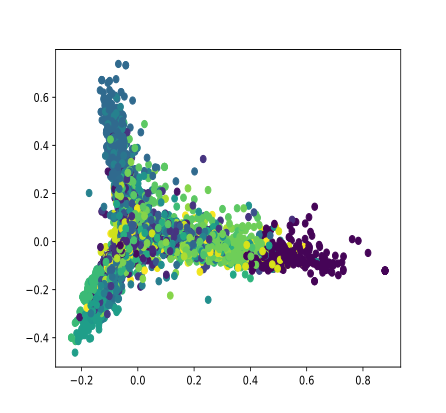
\includegraphics[width=8.5cm]{nlp18}
		\caption{Distribution of Clustering Results}
		\label{nlp18}
	\end{minipage}
\end{figure}
\subsection{Model-based Product Name Inference Results}
\label{sec5.5}
Based on the LDA-K-TF-IDF model, following the ideas mentioned in Section~\ref{sec5.1}, we finally defined the product names in a small but accurate range and deduced the most likely product names. Due to space reasons, we only show the asin code and name of some products, the results are shown in Figure~\ref{nlp19}, and the word cloud map of the overall product name is drawn, as shown in Figure~\ref{nlp20} and~\ref{nlp21}. It can be concluded that the total number of products in Appendix III is 2420, the total number of products in Appendix IV is 900, and most of the products in Appendix III are paper. printer, tape, pencil, calculator and other products, mainly office products, Appendix IV mainly guitar, cable, pedal, tuner, etc., mainly Musical Instruments and their accessories and cables, etc.
\begin{figure}[H]
	\centering
	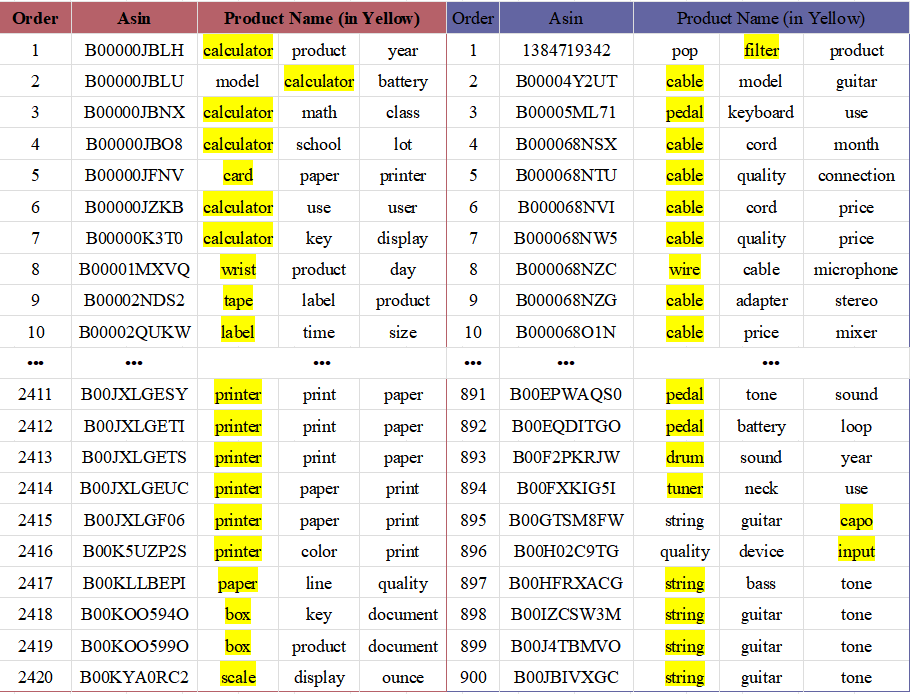
\includegraphics[height=10cm]{nlp19}
	\caption{Appendices 3 and 4 Commodity Name Prediction Results (partial)}
	\label{nlp19}
\end{figure}
\begin{figure}[H]
	\centering
	\begin{minipage}[t]{0.45\linewidth}
		\centering
		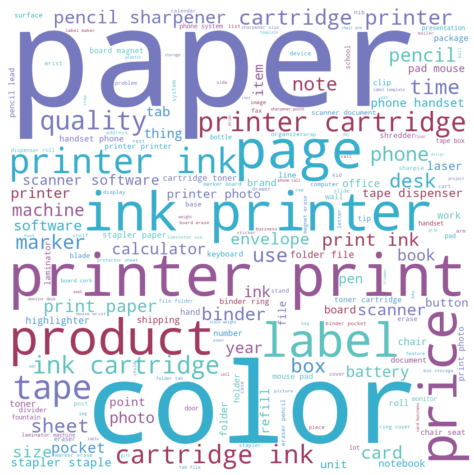
\includegraphics[height=4.2cm]{nlp20}
		\caption{Overall Product Name(3)}
		\label{nlp20}
	\end{minipage}
	\begin{minipage}[t]{0.45\linewidth}
		\centering
		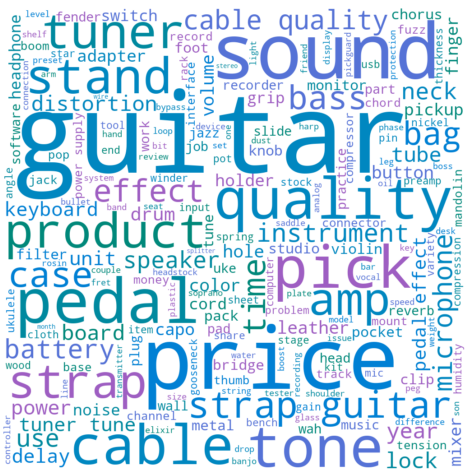
\includegraphics[height=4.2cm]{nlp21}
		\caption{Overall Product Name(4)}
		\label{nlp21}
	\end{minipage}
\end{figure}
\section{Task 3:Sentiment Analysis of Product Reviews}
\subsection{Problem Analysis}
Similar to problem 2, the solution of problem 3 still requires quantification and scoring of words. But the third question is to relate each comment to the corresponding rating. In order to extract keywords from the comments of Appendix V and Appendix VI on the basis of question 2 and further predict product ratings, other appendices should first be used as training sets to extract the comments and rating information preprocessed in question 2, and then combine the two with machine learning algorithms. Apply the trained model to Appendix V and Appendix VI. The prediction accuracy of the model was evaluated by the prediction score and the real score, and the model was improved until a relatively satisfactory answer was obtained.
\begin{figure}[H]
	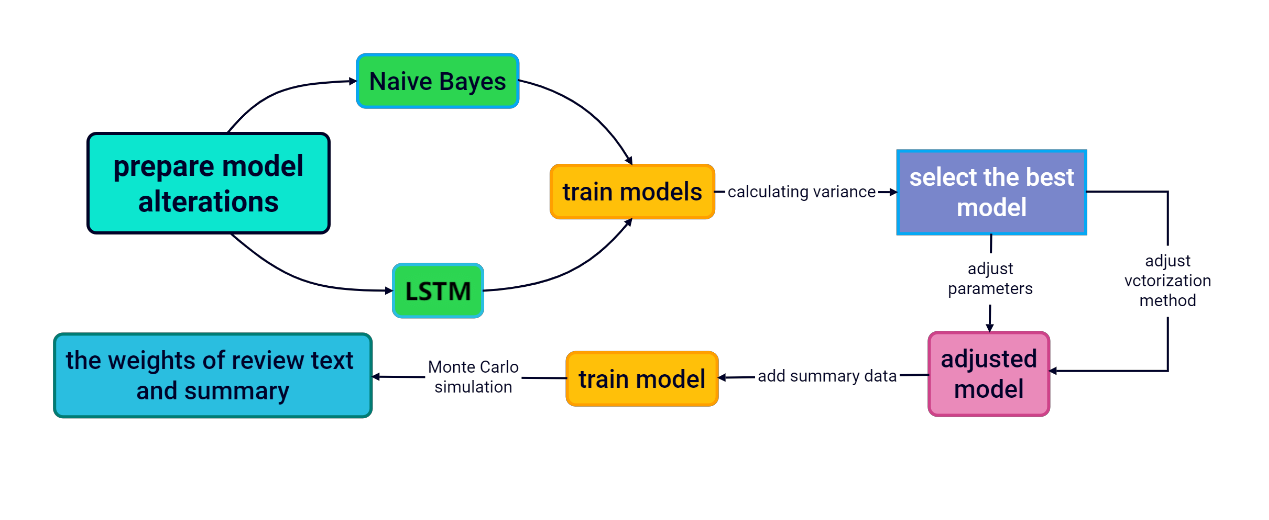
\includegraphics[width=16cm]{nlp22}
	\caption{Task 3 Process}
	\label{nlp22}
\end{figure}
\subsection{LSTM Algorithm}
\subsubsection{Analysis of Model Principle }
\begin{wrapfigure}[10]{l}[0cm]{0pt}
	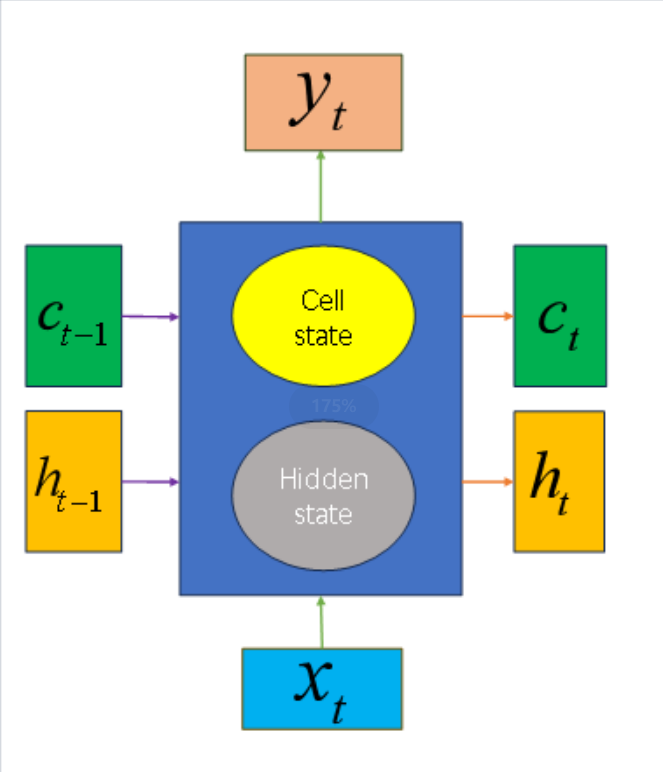
\includegraphics[width=4.7cm]{nlp23}
	\caption{LSTM Cell Diagram}
	\label{nlp23}
\end{wrapfigure}
	Each LSTM unit consists of a forgetting gate, an input gate, an output gate, and a cell, which contains a cell state and a hidden state\cite{5}. And its internal process is mainly divided into three stages:
	
	 1.Forget stage: forgetting door selectively forgets the memory of the previous unit; 

 2.Memory stage: the input data is selectively stored in each cell;

 3.Output stage: Decide to output data and output.\\
	Symbol description:\\
	$x_t$:the input data \qquad $y_t$:the output data\\
	$c_t$:cell state of ‘t’ moment\qquad
	$h_t$:hidden state of ‘t’ moment
\subsubsection{Programming Implementation and Result Analysis}
\label{sec6.2.2}
We used Appendix IV as the training set to train the model. Due to the large amount of total data, and in order to ensure the objective and comprehensive data, we presented the score predictions of the first 30 and the last 30 data in Appendix V.
\begin{figure}[H]
	\centering
	\begin{minipage}[t]{0.45\linewidth}
		\centering
		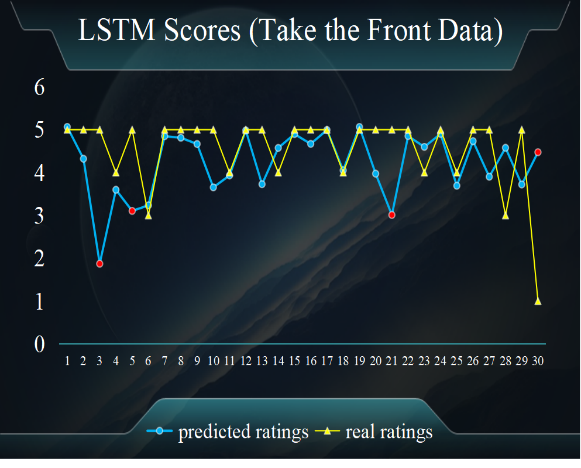
\includegraphics[height=5cm]{nlp24}
		\caption{The First 30 Data}
		\label{nlp24}
	\end{minipage}
	\qquad
	\begin{minipage}[t]{0.45\linewidth}
		\centering
		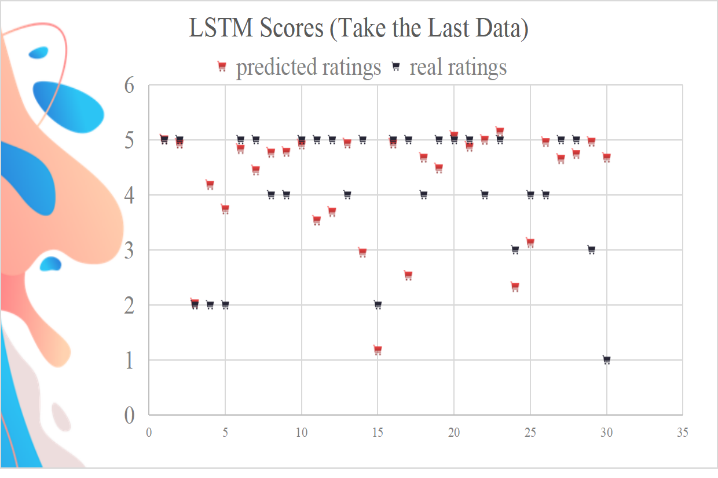
\includegraphics[height=5cm]{nlp25}
		\caption{The Last 30 Data}
		\label{nlp25}
	\end{minipage}
\end{figure}
According to the statistical results, among all 60 pieces of data, 18 pieces of predicted ratings have a deviation greater than 1 from the true value, and 8 pieces have a deviation greater than 2, indicating a large degree of deviation.

It can be observed that the prediction accuracy of the model for the comments with high scores is higher than that for the comments with low scores, which is caused by the small number of low scores in the training set.
\subsection{Naive Bayes}
\subsubsection{Analysis of Model Principle}
The steps of Naive Bayes' learning algorithm are as follows: 
\begin{enumerate}
	\item Prepare data: that is, transform data into a form that can be used for Naive Bayes classification, such as converting text data into numerical feature vectors. Let each sample x in the dataset contain n-dimensional features, and the class tag set contains k categories, i.e. :
	\begin{equation}
		\begin{cases}
			x=(x_1,x_2,\cdots,x_n)\\
			y=(y_1,y_2,\cdots,y_k)
		\end{cases}
	\end{equation}
	\item Training model: Use the training data to estimate the prior probability of each category and the conditional probability of each feature. The Naive Bayes classifier assumes that each feature is independent of each other. According to the above conditions, the Naive Bayes classifier can be expressed as:
	\begin{equation}
		f(x)=\arg_{y_k}\max P(y_k)\times\prod_{i=1}^{n}P(x_i|y_k)
	\end{equation}
	\item Prediction: For each given test sample, the posterior probability of each class is calculated using Bayes' theorem, and the class with the greatest posterior probability is selected as the result.\cite{6}
\end{enumerate}
To assess the accuracy of the forecast we compare the predicted rating with the real rating to calculate the degree of deviation of the prediction. The degree of deviation can be expressed by the following formula:
\begin{equation}
	\bar{E}=\frac{\sum \parallel r_p-r_r\parallel}{n_{data}}
\end{equation}
$r_p$: The predicted score. $r_r$: The true score.$n_{data}$:The total number of predicted scores. 
\subsubsection{Programming Implementation and Result Analysis}
\label{sec6.3.2}
\begin{figure}[h]
	\centering
	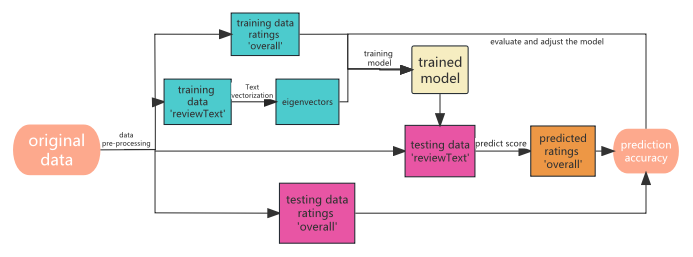
\includegraphics[width=13cm]{nlp26}
	\caption{Program Process}
	\label{nlp26}
\end{figure}
When adjusting Naive Bayes, we give two alternatives for text vectorization and model parameter selection, namely TF-IDF model, bag of words model, and whether to use grid search and cross-validation to get adjusted model parameters. By changing the combination relationship of selection and the amount of data used as the training set, the degree of deviation of prediction results of each group can be obtained. The optimal combination is selected according to the degree of deviation.
\begin{figure}[H]
	\centering
	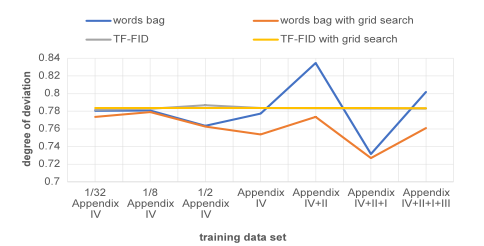
\includegraphics[width=12cm]{nlp27}
	\caption{The Deviation Degree of Four Ways to Implement Naive Bayes}
	\label{nlp27}
\end{figure}
\begin{itemize}
	\item The change in the fluctuation amplitude of group ’words bag’ and ’words bag with grid search’ is due to the sample size of the first three data is small and all come from Appendix Ⅳ, resulting in similar word bags.
	\item In general, TF-IDF had a higher accuracy in prediction than words bag, but the average deviation was similar between the two groups, which may be because the training set and prediction set both used the appendices after removing the stop words, and the advantage of TF-IDF in processing the existing words in the general section was not fully utilized.
	\item The four groups still have relatively low degree of deviation when the training set data is small, indicating that the common advantage of the four groups is that they are not sensitive to the reduction of data.
	\item Overall, combination ‘words bag with grid search’ has the lowest degree of deviation, so the Bayesian sub-model of this combination is selected for subsequent operations.
\end{itemize}
Using the same method as~\ref{sec6.2.2} and applying the model of group‘words bag’, Appendix IV is used as the training set, and the first 30 and last 30 data of Appendix V are used as the test set, resulting in the following charts:
\begin{figure}[H]
	\centering
	\begin{minipage}[t]{0.45\linewidth}
		\centering
		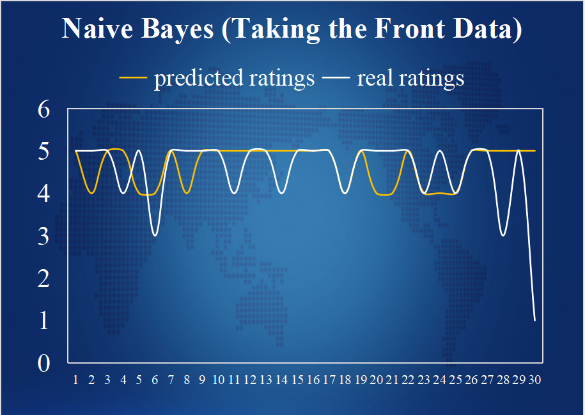
\includegraphics[height=4cm]{nlp28}
		\caption{The First 30 Data}
		\label{nlp28}
	\end{minipage}
	\qquad
	\begin{minipage}[t]{0.45\linewidth}
		\centering
		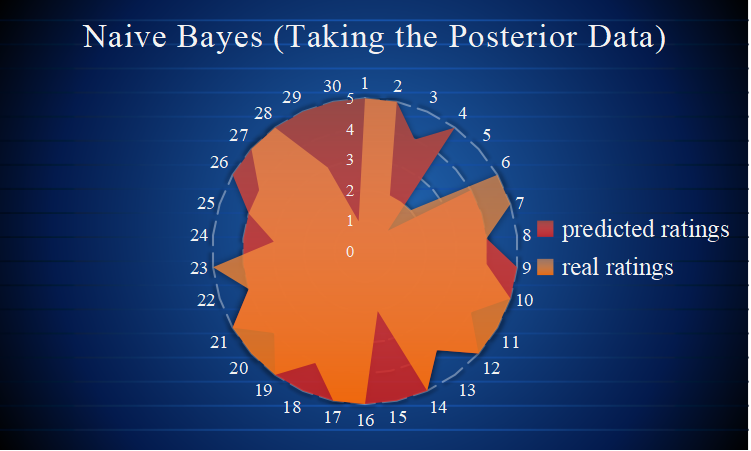
\includegraphics[height=4cm]{nlp29}
		\caption{The Last 30 Data}
		\label{nlp29}
	\end{minipage}
\end{figure}
According to the statistical results, among all 60 pieces of data, 8 pieces of predicted ratings have a deviation greater than 1 from the true value, and 3 pieces have a deviation greater than 2, this shows that the prediction results are relatively accurate.

By observing the radar map on the right, it can be found that the graph area of the predicted value is larger than the graph area of the true value, indicating that the above model has a high prediction of the score.
\subsection{Comparative Analysis and Training Set Correction}
\subsubsection{Comparison and Analysis of Two Models}
Again, we use Appendix IV as training set. And chose the "words bag with grid search" group with the highest prediction accuracy to represent the Naive Bayes model and make the comparison between and LSTM. We used the first 50 pieces of data in Appendix Ⅴ as the test set to evaluate the degree of prediction deviation of the model.
\begin{figure}[H]
	\centering
	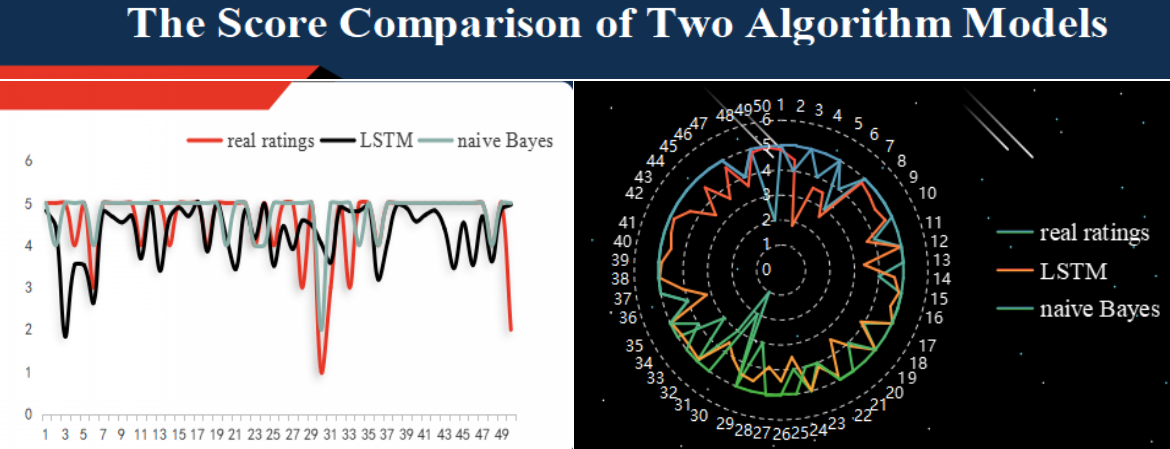
\includegraphics[width=14cm]{nlp30}
	\caption{Comparison of Two Models}
	\label{nlp30}
\end{figure}
\begin{itemize}
	\item It can be seen from the intuitive analysis that the deviation between the prediction results of Naive Bayes model and the true value is smaller than that of LSTM model, and its prediction accuracy is higher than LSTM.
	\item Limited by its own model, Naive Bayes can only predict integer scores, and the predicted scores are concentrated on high scores. Compared with LSTM, Naive Bayes has the disadvantage of being insensitive to different comments.
	\item To sum up, we attach importance to prediction accuracy and choose Naive Bayes algorithm for the next step to ignore the sensitivity of the model to different comments.
\end{itemize}
\subsubsection{Training Set Correction}
Considering that summary can often truly reflect the emotions of reviewers, we obtained two sets of predicted ratings from review text and summary. The weights were assigned to the two sets of data, and Monte Carlo simulation was used to find the weight that minimized the degree of deviation. The sum of the weights of A and B is one.(In order to reduce deviation, we choose the model ’words bag with grid search’ in~\ref{sec6.3.2}).
\begin{figure}[H]
	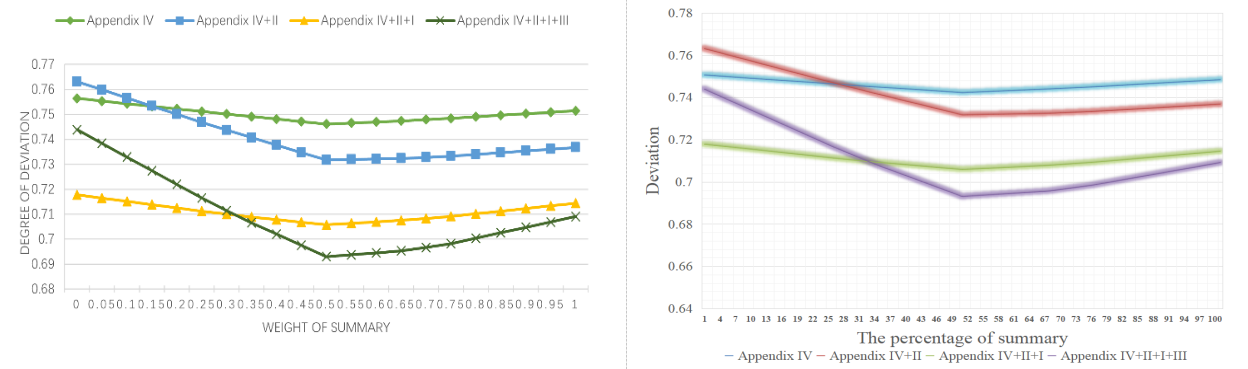
\includegraphics[width=16cm]{nlp31}
	\caption{ Variation of Deviation Degree with Weight or Percentage}
	\label{nlp31}
\end{figure}
\begin{table}[h]
\centering
\caption{Minimum Deviation and Coefficient of Weight}
\resizebox{\textwidth}{15mm}{
\begin{tabular}{ccccc} 
			\toprule[2pt]
			\textbf{Training set}& \textbf{Appendix 4} &\textbf{Appendix 4+2}&\textbf{Appendix 4+2+1} &\textbf{Appendix 4+2+1+3}\\
			\midrule[1pt]
			\textbf{Minimum deviation}& 0.74224&0.7317&0.70579&0.69303\\
			\textbf{Coefficient of weight }& 0.50061&0.50009&0.50041&0.50067\\
			\bottomrule[2pt]
\end{tabular}
}
\end{table}

When the amount of training set data changes greatly, the optimal weights obtained by Monte Carlo simulation are stable at about 0.5, so it can be seen that the optimal weights are constants independent of the amount of training set data.

Compared with only using review text, the prediction deviation degree of Naive Bayes using both summary and review text under optimal weight is significantly negatively correlated with the training data, and has higher prediction accuracy. We did not input more training sets due to the limited amount of data, but it can be seen that this model still has the potential to improve the prediction accuracy.

Even though summary usually contains a small amount of text, it accounts for 0.5 weight in the model, which is consistent with the reality of life. People's views on products are often clearly reflected in summary. Therefore, it is necessary to add summary to the prediction model.
\section{Task 4:Comment Recognition}
\subsection{Model Establishment and Solution}
Our group came up with the following indicators to judge whether a comment is a machine comment: 
\begin{enumerate}
	\item The time of the comment, if a large number of similar comments appear on the same day or several days, then the probability is high. 
	\item Emotional expression of comments and text length, machine comments often use a large number of sentences to express clear emotions.
	\item The richness of sentence syntax, the type of machine sentence syntax is single. 
	\item The degree of correlation between reviews and products, and the probability of generalized reviews is machine reviews. 
\end{enumerate}
\begin{figure}[H]
	\centering
	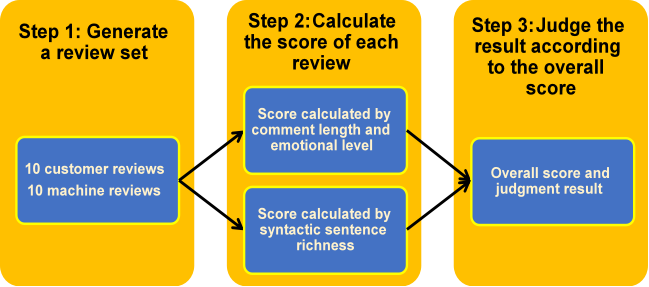
\includegraphics[width=14cm]{nlp32}
	\caption{Program Flow Figure}
	\label{nlp32}
\end{figure}
In order to judge the prediction accuracy of the model and determine the parameters of the model, we collected 10 comments from Appendix Ⅳ as human comments, and then generated 10 machine comments by computer.

In consideration of feasibility, we only consider points 2 and 3 above as criteria. Set the overall score as:
\begin{equation}
	S_p=S_1\times w_1 + S_2\times w_2
\end{equation}
$S_1$: Score by sentiment analysis and text length.\\
$S_2$:Grammar richness score.\\
$w_1, w_2$: The weight obtained by the entropy weight method.

Where $S_1$ can be represented by the following formula:
\begin{equation}
	S_1=\frac{n_s}{\sum \parallel s_e \parallel}
\end{equation}
$s_e$: The emotional value of each sentence obtained by the model of Task Ⅲ. \\
$n_s$: The number of sentences in the review.

By using the context-free method and creating a grammar tree, we scored the sentence syntax richness of paragraph comments. The higher the score, the richer the structure, and the score was recorded as $S_2$.

\subsection{Result Interpretation}
\begin{figure}[H]
	\centering
	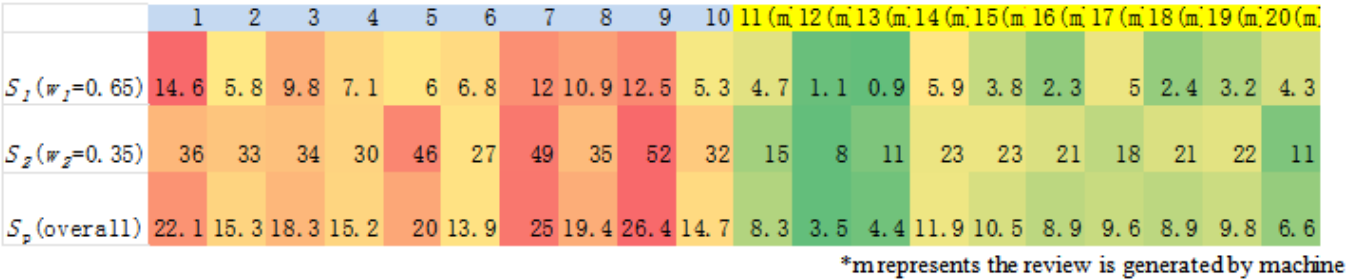
\includegraphics[width=16cm]{nlp33}
	\caption{Score of the Reviews}
	\label{nlp33}
\end{figure}
According to the table, the overall score of the first ten is significantly higher than that of the last ten, which is in line with the expectation, indicating that the model has good judgment ability.

Based on the combined score of each review, we use 12.5 as the criterion, and only reviews with a score higher than 12.5 can be considered customer reviews.

A few of the overall reviews have low scores, which may be due to customers not taking the reviews seriously.
\section{Sensitivity Analysis}
Since other model properties other than problem three are overly dependent on the text content, it is not convenient for us to make quantitative modifications to the text, so here we only perform sensitivity analysis on the modified Naive Bayes model in model three. Our basic idea is to take the data from Appendix Ⅳ, randomly change the 772 'overall' scores to confuse the model's training set, and then use the trained model to score Appendix Ⅵ and calculate the deviation. Then compare the results with the results before the change to determine the stability of the model.
\begin{figure}[H]
	\centering
	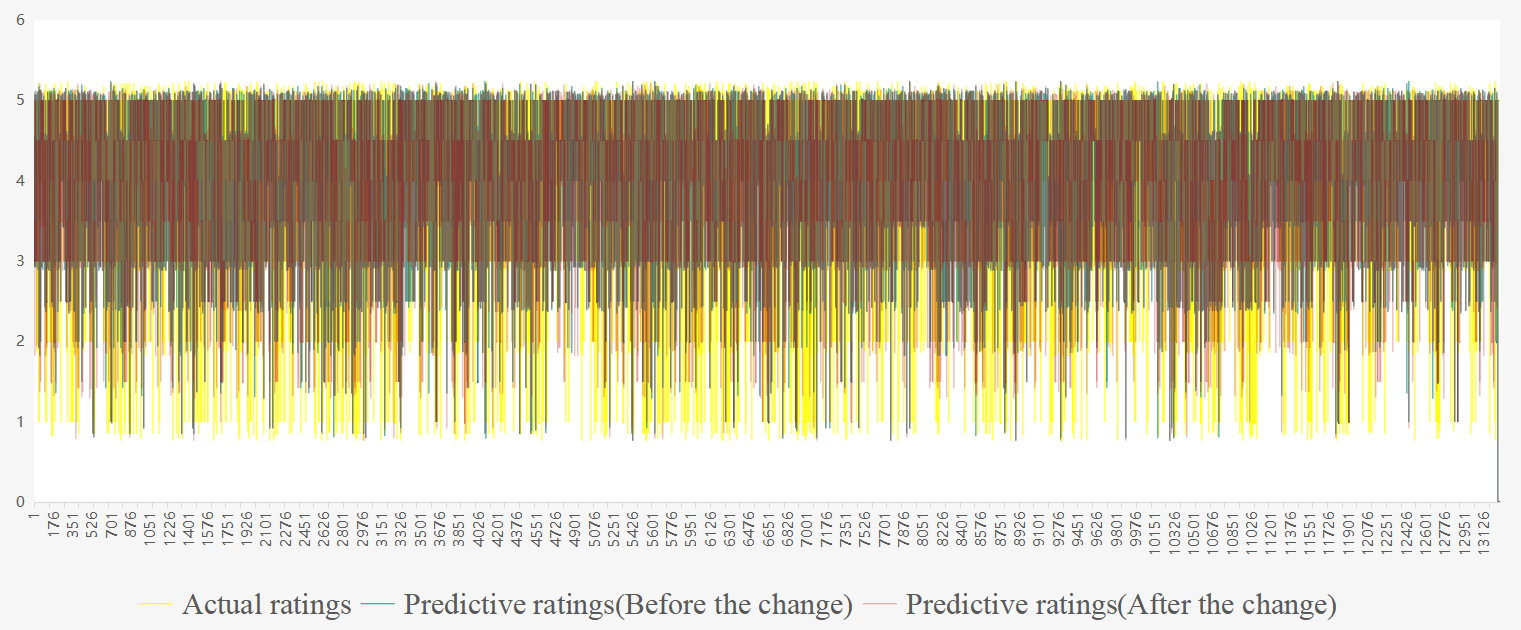
\includegraphics[width=16cm]{nlp34}
	\caption{Change vs. No Change Ratings}
	\label{nlp34}
\end{figure}
As shown in Figure~\ref{nlp34}, qualitative analysis shows that the overall trend of red line and green line is the same and the difference is very small. Monte Carlo quantitative analysis showed that 772 data were randomly changed in the training set of 10260, and the degree of deviation changed from 0.7847929395790902 to 0.8099494606622916, that is, 7.52\% of data confusion only caused the degree of deviation to increase by 3.21\%. So we can conclude that our model has outstanding model stability.

%\begin{Theorem} \label{thm:latex}
%\LaTeX
%\end{Theorem}
%\begin{Lemma} \label{thm:tex}
%\TeX .
%\end{Lemma}
%\begin{proof}
%The proof of theorem.
%\end{proof}

%\lipsum[8] \eqref{aa}
%\begin{equation}
%a^2 \label{aa}
%\end{equation}

\section{Strengths and Weaknesses}
\subsection{Strengths}
\begin{itemize}
\item The LDA-K-TF-IDF model and the naive Bayes model we used are based on solid mathematical principles and are particularly good at dealing with textual data and overcome the limitations of single models;
\item When processing the data and selecting the model, it takes into account a variety of situations, compares the models, and corrects the results in time, which optimizes the analysis results to the greatest extent;
\item Our model has excellent adaptability and can be generalized to more domains, such as feedback on user comments on social media and analysis of general legal texts.
\end{itemize}
\subsection{Weakness}
\begin{itemize}
	\item When using the LDA-K-TF-IDF model to screen product names, it needs to manually adjust the parameters for many times, which leads to a small number of deviations in the results. In the subsequent improvement, the parameters can be objectively weighted to increase the accuracy.
\end{itemize}
\section{Conclusion}
\begin{itemize}
	\item In question 1, we conducted text analysis on Appendix I and Appendix II, obtained high-frequency words after removing stop words and drew word cloud map;
	\item In question 2, we carried out semantic analysis on Appendix III and Appendix IV, and predicted the product names based on LDA-K-TF-IDF model. It was concluded that the former mainly included office products, and the latter mainly included Musical Instruments and their accessories;
	\item In question 3, we conducted sentiment analysis on Appendix 5 and Appendix 6, inferred the commodity rating based on the improved naive Bayes model, and compared with the actual rating, obtained better results;
	\item In Question 4, we establish the criteria to distinguish machine reviews from customer reviews, design algorithms for verification, and write letters to customers to summarize online shopping suggestions.
\end{itemize}
%\subsection{How to cite?}
%bibliography cite use \cite{1,2,3}
%
%AI cite use \AIcite{AI1,AI2,AI3}
\clearpage
\phantomsection 
\addcontentsline {toc} {section} {References}
\begin{thebibliography}{99}
\bibitem{1}Guo J, Ji Y, Woo S, Zhan C. Analyzing E-Commerce Customer Reviews with NLP[J]. Institute for Applied Computational Science, Dec 29, 2020.
\bibitem{2}M Blei D, AndrewY Ng,Michael I.Jordan. LatentDirichlet Allocation[J]. Journal of Machine Learning Research, 2003, 3:993-1022.
\bibitem{3}Zhang Daohai, Yang Chen. Topic Analysis of Logistics Service quality of E-commerce Platform Based on Semantics [J]. Journal of Logistics Science and Technology, 2023,46(1) : 36-40.
\bibitem{4}Sinaga K P, Yang M. Unsupervised K-Means Clustering Algorithm[J]. IEEE Access, 20 April 2020, 8:80716 - 80727.
\bibitem{5}Yu Xiaojian, LIU Guo-peng, LIU Jian-lin, XIAO Wei-Lin. Stocks based on LSTM network and text sentiment analysis[J/OL]. Management Science in China,June 9,2023.
\bibitem{6}Dhaduk H. Performing Sentiment Analysis With Naive Bayes Classifier![J]. Data Science Blogathon, July 13, 2021.
\end{thebibliography}

\begin{appendices}


%\section{First appendix}
%
%In addition, your report must include a letter to the Chief Financial Officer (CFO) of the Goodgrant Foundation, Mr. Alpha Chiang, that describes the optimal investment strategy, your modeling approach and major results, and a brief discussion of your proposed concept of a return-on-investment (ROI). This letter should be no more than two pages in length.
%
%\begin{letter}{Dear, Mr. Alpha Chiang}
%
%\lipsum[1-2]
%
%\vspace{\parskip}
%
%Sincerely yours,
%
%Your friends
%
%\end{letter}
\noindent Here are simulation programmes we used in our model as follow.\\
\textbf{\textcolor[rgb]{0.98,0.00,0.00}{Input python source:}}
\lstinputlisting[language=Python]{./code/123.py}
\lstinputlisting[language=Python]{./code/Kmeans.py}
\lstinputlisting[language=Python]{./code/LDA.py}
\lstinputlisting[language=Python]{./code/lingmin.py}
\lstinputlisting[language=Python]{./code/lingmindu.py}
\lstinputlisting[language=Python]{./code/nameprint.py}
%\newpage
%\begin{minted}{Matlab}
%function [t,seat,aisle]=OI6Sim(n,target,seated)
%pab=rand(1,n);
%for i=1:n
%    if pab(i)<0.4
%        aisleTime(i)=0;
%    else
%        aisleTime(i)=trirnd(3.2,7.1,38.7);
%    end
%end
%\end{minted}
%\section{Second appendix}
%
%some more text \textcolor[rgb]{0.98,0.00,0.00}{\textbf{Input C++ source:}}
%\lstinputlisting[language=C++]{./code/mcmthesis-sudoku.cpp}
%
\end{appendices}
\label{LastPage}
%
%
%\AImatter
%
%\begin{ReportAiUse}{9}
%\bibitem{AI1}
%Bing AI\\
%Query1: write a sort algorithm\\
%Output: Sure, I can help you with that. Here is a simple implementation of the selection sort algorithm in Python:
%\begin{lstlisting}[language=python]
%def selection_sort(arr):
%    for i in range(len(arr)):
%        min_idx = i\part{title}
%        for j in range(i + 1, len(arr)):
%            if arr[min_idx] > arr[j]:
%                min_idx = j
%        arr[i], arr[min_idx] = arr[min_idx], arr[i]
%    return arr
%\end{lstlisting}
%This algorithm sorts an array by repeatedly finding the minimum element from the unsorted part of the array and putting it at the beginning. \href{https://www.geeksforgeeks.org/sorting-algorithms/}{The time complexity of this algorithm is O($n^2$)}.
%
%There are many other sorting algorithms available such as bubble sort, insertion sort, merge sort, quick sort, heap sort, and more. Each of these algorithms has its own advantages and disadvantages. You can learn more about them on GeeksforGeeks and Programiz.
%
%I hope this helps!
%
%\bibitem{AI2}
%OpenAl Enie (Nov 5, 2023 version, Ernie 4.0)\\
%Query1: <insert the exact wording of any subsequent input into the Al tool>\\
%Output: <insert the complete output from the second query>
%
%\bibitem{AI3}
%Github CoPilot (Feb 3, 2024 version)\\
%Query1: <insert the exact wording you input into the Al tool>\\
%Output: <insert the complete output fron the Al tool>
%
%\bibitem{AI4}
%Google Bard (Feb 2,2024 version)\\
%Query: <insert the exact wording of your query>\\
%Output: <irsert the complete output from the Al tool>
%
%\bibitem{AI5}
%Bing AI\\
%Query: write a FFT algorithm\\
%Output: Sure, here is a Python implementation of the Fast Fourier Transform (FFT) algorithm:
%\begin{lstlisting}[language=python]
%import numpy as np
%
%def fft(x):
%    n = len(x)
%    if n == 1:
%        return x
%    even = fft(x[0::2])
%    odd = fft(x[1::2])
%    T = [np.exp(-2j * np.pi * k / n) * odd[k] for k in range(n // 2)]
%    return [even[k] + T[k] for k in range(n // 2)] + [even[k] - T[k] for k in range(n // 2)]
%\end{lstlisting}
%The FFT is a widely used algorithm for computing the \textbf{Discrete Fourier Transform (DFT)} of a sequence. It reduces the number of computations needed from O(n$^2$) to O(n log n) 12. The basic idea of the FFT is to apply divide and conquer. We divide the coefficient vector of the polynomial into two vectors, recursively compute the DFT for each of them, and combine the results to compute the DFT of the complete polynomial 3.
%
%I hope this helps!
%
%\end{ReportAiUse}
\end{document}
%% 
%% This work consists of these files mcmthesis.dtx,
%%                                   figures/ and
%%                                   code/,
%% and the derived files             mcmthesis.cls,
%%                                   mcmthesis-demo.tex,
%%                                   README,
%%                                   LICENSE,
%%                                   mcmthesis.pdf and
%%                                   mcmthesis-demo.pdf.
%%
%% End of file `mcmthesis-demo.tex'.
